\section{Serie numeriche} 
\subsection{Introduzione}

\begin{gather*}
	\sin x = \sum_{k=0}^{\infty} (-1)^{k} \frac{x^{2k+1}}{(2k+1)!}
	\\
	\sin 4 = \sum_{k=0}^{\infty} (-1)^{k} \frac{4^{2k+1}}{(2k+1)!} = 
	4 - \frac{4^3}{3!} + \frac{4^5}{5!} - \frac{4^7}{7!} + \ldots 
	\\
	\sum_{k=1}^{\infty} \frac{1}{k} = 1 + \frac{1}{2} + \frac{1}{3} + \frac{1}{4} + \frac{1}{5} + \ldots = +\infty
	\\
	\sum_{k=1}^{5} \frac{1}{k} = 1 + \frac{1}{2} + \frac{1}{3} + \frac{1}{4} + \frac{1}{5} 
	\\
	\sum_{k=1}^{10} \frac{1}{k} = 1 + \frac{1}{2} + \frac{1}{3} + \ldots + \frac{1}{10}
	\\
	\sum_{k=1}^n \frac{1}{k} = 1 + \frac{1}{2} + \frac{1}{3} + \ldots + \frac{1}{n} \qquad n \geq 1 
	\\
	\sum_{k=1}^{\infty} \frac{1}{k} = \lim_{n\rightarrow\infty} \sum_{k=1}^{n} \frac{1}{k} 
\end{gather*}


\begin{definition} 
	Una serie a valori in $\mathbb{C}$ è una coppia $(\{a_n\}_{n \in \mathbb{N}}, \{S_n\}_{n\in\mathbb{N}})$ tale che $\{a_n\}_{n\in\mathbb{N}} \subseteq \mathbb{C}$ è una successione e $\{S_n\}_{n\in\mathbb{N}}$ è la successione delle ridotte.
	$S_n=\sum_{k=0}^{n} a_k$ si dice ridotta n-esima.
\end{definition}


\begin{exbar} 
	\begin{gather*}
		S_0=a_0 \qquad S_1=a_0+a_1 \qquad	S_2=a_0+a_1+a_2 \\
		S_3=a_0+a_1+a_2+a_3 \qquad \ldots \qquad S_n=a_0+a_1+\ldots+a_n
	\end{gather*}
\end{exbar}

La coppia $(\{a_n\}_{n \in \mathbb{N}}, \{S_n\}_{n\in\mathbb{N}})$ è identificata con $\sum_{k=0}^{\infty} a_k$

\begin{definition}
	Una serie $\sum_{k=0}^{\infty} a_k$ si dice:
	\begin{enumerate}
		\item \textbf{Convergente} se converge la successione delle ridotte, cioè se $\exists$ finito
		
		$\lim_{n\rightarrow+\infty} S_n = \lim_{n\rightarrow+\infty} \sum_{k=0}^{n} a_k$
		
		\item \textbf{Divergente} 
		\begin{enumerate}
			\item a $+\infty$ se $\lim_{n\rightarrow+\infty} S_n = +\infty$
			\item a $-\infty$ se $\lim_{n\rightarrow+\infty} S_n = -\infty$
			\item a $\infty$ se $\lim_{n\rightarrow+\infty} S_n = \infty$, cioè se $\lim_{n\rightarrow+\infty} |S_n| = +\infty$
		\end{enumerate}
		
		\item  \textbf{Irregolare o indeterminata} se $\lim_{n\rightarrow+\infty} S_n$ non esiste.
	\end{enumerate}
\end{definition}

\begin{exbar}
	$\sum_{k=0}^\infty (-1)^k \frac{4^{2k+1}}{(2k+1)!} = \lim_{n\rightarrow+\infty} \sum_{k=0}^n (-1)^k \frac{4^{2k+1}}{(2k+1)!} = \sin(4)$ è convergente;
	
	$\sum_{k=1}^\infty \frac{1}{k} = \lim_{n\rightarrow+\infty}\sum_{k=1}^n = +\infty$ è divergente. 
\end{exbar}

\begin{definition}
	Se la serie $\sum_{k=0}^{\infty} a_k$ converge, il $\lim_{n\rightarrow+\infty} S_n = \lim_{n\rightarrow+\infty} \sum_{k=0}^{n} a_k$ si dice somma della serie ed è indicato con $\sum_{k=0}^\infty a_k$
\end{definition}

\begin{proposition}
	\label{prop:serie complessa}
	Sia $\sum_{k=0}^\infty a_k$ una serie a termini complessi. Allora $\sum_{k=0}^\infty a_k$ converge $\iff$ convergono $\sum_{k=0}^\infty \mathrm{Re}(a_k)$ e $\sum_{k=0}^\infty \mathrm{Im}(a_k)$
\end{proposition}

\begin{exbar}
	$a_k = \alpha_k + i \beta_k$ \qquad $\alpha_k$, $\beta_k\in\mathbb{R}$ \qquad $\alpha_k = \mathrm{Re}(a_k)$, $\beta_k = \mathrm{Im}(a_k)$
	
	$\sum_{k=0}^\infty a_k$ converge $\iff$ convergono entrambe le serie a termini in $\mathbb{R}$ $\sum_{k=0}^\infty \alpha_k$ e $\sum_{k=0}^\infty \beta_k$.
\end{exbar}

Della serie è interessante studiare il carattere, cioè se convergono, divergono o sono irregolari.

\begin{dembar}
	\textbf{Dimostrazione} della \textbf{Proposizione \ref{prop:serie complessa}} 
	\begin{itemize}
		\item \textit{Condizione sufficiente $(\Rightarrow)$}: $\sum_{k=0}^\infty a_k$ converge $\Rightarrow \sum_{k=0}^\infty \alpha_k$ e $\sum_{k=0}^\infty \beta_k$ convergono. 
		
		Sia $S_a + iS_b$ la somma di $\sum_{k=0}^\infty a_k$, $S_a + iS_b = \lim_{n\rightarrow+\infty} \sum_{k=0}^n (\alpha_k + i\beta_k)$.
		
		Faccio vedere che $\lim_{n\rightarrow+\infty} \sum_{k=0}^n \alpha_k = S_a$ e $\lim_{n\rightarrow+\infty} \sum_{k=0}^n \beta_k = S_b$.
		
		$0 \leq \biggl|\sum_{k=0}^n \alpha_k - S_a \biggr| = \biggl|\mathrm{Re}(\sum_{k=0}^n a_k - (S_a + iS_b)) \biggr| \leq \biggl| \sum_{k=0}^n a_k - (S_a + iS_b) \biggr| \rightarrow 0$ per $n\rightarrow+\infty$
		
		Per il teorema del confronto $\lim_{n\rightarrow+\infty} \biggl| \sum_{k=0}^n \alpha_k -S_a \biggr| = 0 \iff \lim_{n\rightarrow+\infty} \sum_{k=0}^n \alpha_k = S_a$.
		
		In modo analogo si dimostra che $\lim_{n\rightarrow+\infty} \sum_{k=0}^n \beta_k = S_b$.
		
		\vspace{5pt}
		
		\item \textit{Condizione necessaria $(\Leftarrow)$}: 
		$\sum_{k=0}^\infty \alpha_k$ e $\sum_{k=0}^\infty \beta_k$ convergono $\Rightarrow$ $\sum_{k=0}^\infty a_k$ converge. 
		
		\begin{equation*}
			\lim_{n\rightarrow+\infty} \sum_{k=0}^n \alpha_k = S_a \in \mathbb{R} \qquad \lim_{n\rightarrow+\infty} \sum_{k=0}^n \beta_k = S_b \in \mathbb{R}
		\end{equation*}
		\begin{align*}
			0 \leq \biggl| \sum_{k=0}^n a_k - (S_a + iS_b) \biggr|
			&= \biggl| (\sum_{k=0}^n \alpha_k -S_a) + i(\sum_{k=0}^n \beta_k - S_b) \biggr| \\
			& \distr \biggl| \sum_{k=0}^n \alpha_k -S_a) \biggr| + \biggl| \sum_{k=0}^n \beta_k - S_b \biggr| \xrightarrow{n\rightarrow+\infty}  0 
		\end{align*}
		
		e si conclude con il teorema del confronto. $\square$
	\end{itemize}
\end{dembar}


\subsubsection{Paradosso di Zenone} 
\begin{figure}[!h]
	\centering
	\includegraphics[width=0.7\linewidth]{zenone}
	\caption{Paradosso di Zenone}
	\label{fig:zenone}
\end{figure}

A Achille, T tartaruga, $v_A>v_T$ 

\begin{align*}
\centering
L_0 & \qquad t_0 = \frac{L_0}{v_A} 
\\
L_1=t_0\cdot v_T & \qquad t_1=\frac{L_1}{v_A} = t_0\frac{v_T}{v_A}
\\
L_2=t_1\cdot v_T & \qquad t_2=\frac{L_2}{v_A} = t_1 \frac{v_T}{v_A} = t_0 \biggl( \frac{v_T}{v_A} \biggr) ^2 
\\
L_3=t_2\cdot v_T & \qquad t_3=\frac{L_3}{v_A} =  t_0 \biggl( \frac{v_T}{v_A} \biggr) ^3
\end{align*}
Quanto tempo impiega Achille a raggiungere la tartaruga?

\newcommand\zenone{\stackrel{\mbox{\tiny{$v_T<v_A$}}}{=}}

\begin{align*}
	T   &= t_0 + t_1 + t_2 + \ldots = t_0 \biggl(1 + \frac{v_T}{v_A} + \biggl(\frac{v_T}{v_A}\biggr)^2 + \ldots + \biggl(\frac{v_T}{v_A}\biggr)^n + \ldots \biggr)	= t_0 \sum_{k=0}^\infty \biggl(\frac{v_T}{v_A}\biggr)^k = \\
	&\zenone t_0 \frac{1}{1-\frac{v_T}{v_A}} = \frac{\frac{L_0}{v_A}}{1-\frac{v_T}{v_A}}
\end{align*}

\subsubsection{Serie geometrica} di ragione r, con $r\in\mathbb{C}$

\begin{equation*}
	\sum_{k=0}^\infty r^k = r^0 + r^1 + r^2 + \ldots
\end{equation*}

\begin{itemize}
	\item $r=1$
	\begin{align*}
		\sum_{k=0}^\infty 1^k
		&= \lim_{n} \sum_{k=0}^n 1^k = \lim_{n} \underbrace{(1 + 1 + \ldots +1)}_\text{n+1 volte} = \\
		&=\lim_{n} (n+1) = +\infty
	\end{align*}
	
	\item $r\neq1$ \qquad Procuriamoci un'espressione della ridotta n-esima, cioè 
	\begin{equation*}
		S_n = \sum_{k=0}^n r^k = 1 + r + r^2 + \ldots + r^n
	\end{equation*}
	
	\begin{gather*}
		\begin{cases*}
			S_{n+1} = \sum_{k=0}^{n+1} r^k = \underbrace{1 + r + r^2 + \ldots + r^n}_\text{$S_n$} + r^{n+1} = S_n + r^{n+1} \\
			S_{n+1} = 1 + \underbrace{r + r^2 +r^3 + \ldots + r^n + r^{n+1}}_\text{raccolgo r a fattore comune} = 1 + r(1 + r + r^2 + \ldots + r^n) = 1 + rS_n
		\end{cases*}  \Rightarrow
		\\
		\Rightarrow S_n + r^{n+1} = 1 + rS_n
	\end{gather*}
	

	
	\begin{equation}
		S_n = \frac{1 - r^{n+1}}{1-r}
	\end{equation}
\end{itemize}

\begin{exbar}
	Per Achille e la Tartaruga $r=\frac{v_T}{v_A}$.
\end{exbar}

\begin{attbar}
	$\lim_{n} S_n = \lim_{n} \frac{1-r^{n+1}}{1-r} \exists$ finito e vale in tal caso $\frac{1}{1-r} \iff |r|<1$
\end{attbar}

\begin{attbar}
	La serie geometrica di ragione $r$, $\sum_{k=0}^\infty r^k$ converge $\iff |r|<1$ e in tal caso la sua somma vale $\frac{1}{1-r}$.
\end{attbar}

\begin{exbar}
	\begin{example} Dimostriamo che $0.\bar{9} = 1$
		\begin{align*}
			0.\bar{9} 
			&= \sum_{k=1}^\infty \frac{9}{10^k} = \lim_{n\rightarrow+\infty} \sum_{k=1}^n \frac{9}{10^k} = 9 \lim_{n\rightarrow+\infty} \sum_{k=1}^n \frac{1}{10^k} = 9 \lim_{n\rightarrow+\infty} \biggl( \sum_{k=0}^n \frac{1}{10^k} - \frac{1}{10^0} \biggr) = \\
			&= 9 \biggl( \sum_{k=0}^\infty \biggl(\frac{1}{10} \biggr)^k - 1 \biggr) = 9 \biggl( \frac{1}{1-\frac{1}{10}} -1 \biggr) = 9 \biggl( \frac{10}{9} -1 \biggr) = \\
			&=1
		\end{align*}	
	\end{example}
\end{exbar}

\subsubsection{Serie telescopiche}
\begin{equation*}
	\sum_{k=0}^\infty [f(k+1) - f(k)] \qquad f:\mathbb{N}\rightarrow\mathbb{C}
\end{equation*}


Studiamo il carattere. Procuriamoci, se possibile, l'espressione di una ridotta n-esima
\begin{align*}
	S_n &= \sum_{k=0}^n [f(k+1)-f(k)] = \\
	&= \overbrace{\cancel{f(1)}-f(0)}^{k=0} + \overbrace{\cancel{f(2)}-\cancel{f(1)}}^{k=1} + \overbrace{\cancel{f(3)}-\cancel{f(2)}}^{k=2} +  \overbrace{\cancel{f(4)}-\cancel{f(3)}}^{k=3} + \ldots + \overbrace{f(n+1)-\cancel{f(n)}}^{k=n} = \\
	&= f(n+1) -f(0)
\end{align*}
\begin{attbar}
	$\lim_{n}S_n = \lim_{n}[f(n+1)-f(0)]$ esiste $\iff$ esiste $\lim_{n} f(n)$.
	
	La serie converge $\iff$ $\lim_{n} f(n)$ esiste finito e in tal caso la somma della serie è 
	\begin{equation*}
			\sum_{k=0}^\infty [f(k+1)-f(k)] = \lim_{n\rightarrow+\infty} f(n)-f(0)
	\end{equation*}

\end{attbar}

\begin{exbar}
	\begin{example} (serie di Mengoli)
		\begin{align*}
			\sum_{k=1}^\infty \frac{1}{k(k+1)} 
			&= \sum_{k=1}^\infty \biggl( \frac{1}{k} -\frac{1}{k+1} \biggr) \\
			&= -\sum_{k=1}^\infty \biggl[\frac{1}{k+1} - \frac{1}{k}\biggr] & \mathrm{dove} \, \frac{1}{k}=f(k) \\
			&= -\lim_{n}[f(n)-f(1)] = f(1) = \\
			&= 1
		\end{align*}
	\end{example}
\end{exbar}

\subsubsection{Formula di Eulero} 

\begin{gather*}
	e^{i\theta} = \cos(\theta) + i \sin(\theta) 
	\\	
	e^{in\theta} = \cos(n\theta) + i\sin(n\theta)
	\\	
	\sum_{n=0}^\infty [\cos(n\theta)+i\sin(n\theta)] = \sum_{n=0}^\infty e^{in\theta} =  \sum_{n=0}^\infty (e^{i\theta})^n
\end{gather*}
Non converge, perché è una serie geometrica di ragione $e^{i\theta}$ e $|e^{i\theta}| = 1$.

Se $\theta = 0, 2\pi$:
\begin{itemize}
	\item $\sum_{n=0}^\infty \cos(n\theta) = \sum_{n=0}^\infty 1 = +\infty$
	\item $\sum_{n=0}^\infty \sin(n\theta) = \sum_{n=0}^\infty 0 = 0$
\end{itemize}

Se $\theta \neq 0, 2\pi$:
\begin{itemize}
	\item $\sum_{k=0}^n \cos(k\theta) = \mathrm{Re} \bigg(\sum_{k=0}^n (e^{i\theta})^k \bigg) = \mathrm{Re} \bigg( \frac{1-e^{i\theta(n+1)}}{1-e^{i\theta}} \bigg)$
	\item $\sum_{k=0}^n \sin(k\theta) = \mathrm{Im} \bigg(\sum_{k=0}^n (e^{i\theta})^k \bigg) = \mathrm{Im} \bigg( \frac{1-e^{i\theta(n+1)}}{1-e^{i\theta}} \bigg)$
\end{itemize}

\begin{align*}
	& \qquad \frac{1-e^{i\theta(n+1)}}{1-e^{i\theta}} \\
	&= \frac{1 - \cos[(n+1)\theta] - i \sin[(n+1)\theta]}{1-\cos\theta - i \sin\theta} \\
	&= \frac{1 - \cos[(n+1)\theta] - i\sin[(n+1)\theta]}{|1-\cos\theta-i\sin\theta|^2} \cdot (1 - \cos\theta + i\sin\theta) \\
	&= \frac{1}{2(1-\cos\theta)} \cdot \{1 - \cos[(n+1)\theta] - i\sin[(n+1)\theta]\} \cdot (1 - \cos\theta + i\sin\theta)= \\
	&= \frac{1}{2(1-\cos\theta)} \cdot \{ 1 - \cos\theta - \cos[(n+1)\theta] + \cos\theta\cos[(n+1)\theta] + \sin\theta\sin[(n+1)\theta] + \\
	& \quad + i[\sin\theta-\cos[(n+1)\theta]\sin\theta - \sin[(n+1)\theta] + \sin[(n+1)\theta] \cos\theta ] \}
\end{align*}

Separiamo parte reale e immaginaria e raccogliamo:
\begin{gather*}
	\sum_{k=0}^n \cos(k\theta) =  \frac{1}{2(1-\cos\theta)} \cdot [(1-\cos\theta)(1-\cos((n+1)\theta)) + \sin\theta\sin((n+1)\theta)]
	\\
	\sum_{k=0}^n \sin(k\theta) =  \frac{1}{2(1-\cos\theta)} \cdot [\sin\theta(1-\cos((n+1)\theta)) - \sin((n+1)\theta)(1-\cos\theta)]
\end{gather*}	
	
	
\subsection{Studio del carattere di una serie}
\begin{theorem}
	\label{th:termine generale}
	$\{a_k \}_{k\in\mathbb{N}} \subseteq \mathbb{C}$ $($oppure $\mathbb{R})$. Se $\sum_{k=0}^\infty a_k$ converge, allora $\lim_{k\rightarrow+\infty} a_k = 0$.
\end{theorem}
Se una serie è convergente il suo termine generale è infinitesimo.

\begin{exbar}
	\begin{example} (serie armonica)
		
		\textbf{Non è vero} che $\lim_{k\rightarrow+\infty} a_k = 0 \Rightarrow \sum_{k=0}^\infty a_k$ converge.
		
		$\sum_{k=1}^\infty \frac{1}{k}$ serie armonica diverge, ma $\lim_{k\rightarrow+\infty}\frac{1}{k} = 0$.
		
		Prendiamo $x$ compresa tra due numeri interi $k$ e $k+1$, con $k\geq 1$.
		\begin{gather*}
			k\leq x \leq k+1
			\\
			\frac{1}{k+1} \leq \colorbox{yellow}{\parbox{1.1cm}{$\frac{1}{x} \leq \frac{1}{k}$}}
			\\
			\int_{k}^{k+1} \frac{1}{x} \mathrm{d}x \leq \int_{k}^{k+1} \frac{1}{k} \mathrm{d}x = \frac{1}{k}
			\\
			\frac{1}{k} \geq \int_{k}^{k+1} \frac{1}{x} \mathrm{d}x = \ln(k+1) -\ln(k)
			\\
			\sum_{k=1}^n \frac{1}{k} \geq \sum_{k=1}^n [\ln(k+1)-\ln(k)] = \ln(n+1)-\ln(1) = \ln(n+1) 
		\end{gather*}
		
		Per il teorema del confronto $\lim_{n}\sum_{k=0}^n \frac{1}{k} \geq \lim_{n} \ln(n+1) = +\infty \Rightarrow \sum_{k=1}^\infty \frac{1}{k} = +\infty$.
	\end{example}
\end{exbar}

\begin{attbar}
	Il \textbf{Teorema \ref{th:termine generale}} si può rileggere: se $\lim_{k\rightarrow+\infty} a_k \neq 0 \Rightarrow \sum_{k=0}^\infty a_k$ non converge.
\end{attbar}

Riprendendo l'esempio del paragrafo precedente vediamo che i termini generale di $\sin(k\theta)$ e $\cos(k\theta)$ non esistono: $\lim_{k\rightarrow+\infty} \cos(k\theta)$ non esiste se $\theta \neq \frac{\pi}{2}, \frac{3\pi}{2}$ e $\lim_{k\rightarrow+\infty} \sin(k\theta)$ non esiste se $\theta\neq 0, 2\pi$.

\begin{dembar}
	\textbf{Dimostrazione} del \textbf{Teorema \ref{th:termine generale}} 
	
	Sappiamo che $\sum_{k=0}^\infty a_k$ converge.
	
	\begin{gather*}
		S_n = \sum_{k=0}^n a_k \qquad S_{n-1} = \sum_{k=0}^{n-1} a_k
		\\
		S_n - S_{n-1} = \sum_{k=0}^n a_k - \sum_{k=0}^{n-1} a_k = a_n + \sum_{k=0}^{n-1} a_k - \sum_{k=0}^{n-1} a_k = a_n
		\\
		\lim_{n} a_n = \lim_{n} (\vertarrowbox{S_n}{$S$} - \vertarrowbox{S_{n-1}}{$S$}) = 0 
	\end{gather*}
	
	$S\in\mathbb{C}$ somma della serie. $\square$
\end{dembar}

\begin{proposition}
	\label{prop:somma convergenti}
	Siano $\sum_{n=0}^\infty a_n$ e $\sum_{n=0}^\infty b_n$ serie convergenti di somma $S_a$ ed $S_b$ rispettivamente. Allora $\sum_{n=0}^\infty (a_n + b_n)$ converge e la sua somma è $S_a+S_b$
\end{proposition}

\begin{dembar}
	\textbf{Dimostrazione} della \textbf{Proposizione \ref{prop:somma convergenti}}
	
	\begin{equation*}
		\sum_{k=0}^n (a_k + b_k) = \vertarrowbox{\sum_{k=0}^\infty a_k}{$S_a$} + \vertarrowbox{\sum_{k=0}^\infty b_k}{$S_b$} \xrightarrow{n\rightarrow+\infty} S_a + S_b \quad \square 
	\end{equation*}
	
\end{dembar}

\begin{proposition}
	\label{prop:prodotto convergente}
	Sia $\sum_{k=0}^\infty a_k$ serie convergente di somma S e sia $c\in\mathbb{C}$. Allora $\sum_{k=0}^\infty (c \cdot a_k)$ converge e la sua somma è $c \cdot S$
\end{proposition}

\begin{dembar}
	\textbf{Dimostrazione} della \textbf{Proposizione \ref{prop:prodotto convergente}}
	\begin{equation*}
		\sum_{k=0}^n (c\cdot a_k) = c\vertarrowbox{\sum_{k=0}^n a_k}{$S$} \xrightarrow{n\rightarrow+\infty} c\cdot S \quad \square
	\end{equation*}

\end{dembar}

\begin{proposition}
	\label{prop:stesso carattere}
	Sia data la serie $\sum_{k=0}^\infty a_k$ e sia $n_0\in\mathbb{N}$, $n_0\geq1$. Allora $\sum_{k=0}^\infty a_k$ e $\sum_{k=n_0}^\infty a_k$ hanno lo stesso carattere.
\end{proposition}

\begin{exbar}
	$\sum_{k=1}^\infty \frac{1}{k}$ e $\sum_{k=10^{10}}^\infty \frac{1}{k}$ hanno lo stesso carattere, quindi $\sum_{k=10^{10}}^\infty \frac{1}{k} = +\infty$.
\end{exbar}

\begin{attbar}
	Il carattere di una serie dipende solo dalla coda della successione dei suoi termini.
\end{attbar}

\begin{dembar}
	\textbf{Dimostrazione} della \textbf{Proposizione \ref{prop:stesso carattere}}
	
	Sia $n_0<n$ e $\sum_{k=0}^n a_k = \sum_{k=0}^{n_0-1} a_k + \sum_{k=n_0}^n a_k$
	
	$\lim_{n} \sum_{k=0}^n a_k$ esiste $\iff \exists \lim_{n\rightarrow+\infty} \sum_{k=n_0}^n a_k$ per la \textbf{Proposizione \ref{prop:somma convergenti}} e in tal caso 
	
	$\lim_{n} \sum_{k=0}^n a_k = \bigg(\lim_{n} \sum_{k=n_0}^n a_k \bigg) + \bigg(\sum_{k=0}^{n_0-1}a_k\bigg). \quad \square$
\end{dembar}

\begin{definition}
	Sia $\{a_n\}_{n\in\mathbb{N}}$ successione in $\mathbb{R}$ o in $\mathbb{C}$. Allora $\{a_n\}_{n\in\mathbb{N}}$ si dice di Cauchy se $\forall \; \varepsilon > 0 \; \exists \; N>0 \mid \forall \; n>N$ e $p\geq0$ \quad $\mid a_{n+p} - a_n \mid < \varepsilon$.
\end{definition}

\begin{theorem} (criterio di Cauchy per le successioni)
	Sia $\{a_n\}_{n\in\mathbb{N}}$ successione in $\mathbb{R}$ o in $\mathbb{C}$. Allora $\{a_n\}_{n\in\mathbb{N}}$ è convergente $\iff$ è di Cauchy
\end{theorem}

\begin{theorem} (criterio di Cauchy per le serie)
	\label{th:Cauchy serie}
	Sia data una serie $\sum_{k=0}^\infty a_k$ in $\mathbb{R}$ o in $\mathbb{C}$. Allora la serie converge $\iff \forall \; \varepsilon > 0 \; \exists \; N>0 \; \mid$ se $n>N$ e $p\geq0$ \quad $\biggl| \sum_{k=n}^{n+p} a_k \biggr| < \varepsilon$.
\end{theorem}

{\noindent Si ricava dal criterio di Cauchy per le successioni osservando che $\sum_{k=n}^{n+p} a_k = S_{n+p} - S_{n-1}$ \par}

\begin{proposition}
	\label{prop:no indeterminata}
	Sia $\sum_{k=0}^\infty a_k$ serie a termini definitivamente non negativi $\mathrm{(} \exists \; N>0 \; | \; a_k\geq 0 \; \forall \; k>N \mathrm{)}$. Allora la serie converge o diverge, non può essere indeterminata. 
\end{proposition}

\begin{dembar}
	\textbf{Dimostrazione} della \textbf{Proposizione \ref{prop:no indeterminata}}
	
	Per semplicità assumiamo $a_k \geq 0 \; \forall \; k\in\mathbb{N}$. Devo far vedere che, se $\{S_n \}_{n\in\mathbb{N}}$ è la successione delle ridotte, questa fa limite finito o infinito.
	\begin{equation*}
		S_{n+1} = \sum_{k=0}^{n+1} a_k = a_{n+1} + \sum_{k=0}^n = \vertarrowbox{a_{n+1}}{$\geq 0$} + S_n \geq S_n
	\end{equation*}
	
	$\{S_n \}_{n\in\mathbb{N}}$ è crescente e quindi fa limite finito o a $+\infty$. \quad $\square$
\end{dembar}

\begin{theorem}
	\label{th:convergenza assoluta}
	Sia data la serie $\sum_{k=0}^\infty a_k$ e si supponga che $\sum_{k=0}^\infty |a_k|$ converga (si dice che $\sum_{k=0}^\infty a_k$ converge assolutamente). Allora anche $\sum_{k=0}^\infty a_k$ converge e in tal caso $\bigg| \sum_{k=0}^\infty a_k \biggr| \leq \sum_{k=0}^\infty |a_k|$.
\end{theorem}

\begin{dembar}
	\textbf{Dimostrazione} del \textbf{Teorema \ref{th:Cauchy serie}}
	
	Siccome $\sum_{k=0}^\infty |a_k|$ converge, $\forall \; \varepsilon>0 \; \exists \; N>0 \; | $ se $n>N$ e $p\geq 0$ \quad $\sum_{k=n}^{n+p} |a_k| < \varepsilon$
	
	$\bigg| \sum_{k=n}^{n+p} a_k \bigg| \distr \sum_{k=n}^{n+p} |a_k| < \varepsilon$ se $n>N$ e $p\geq0 \Rightarrow$ la serie soddisfa la condizione di Cauchy e quindi converge.
	
	In tal caso 
	\begin{align*}
		\bigg| \sum_{k=0}^\infty a_k \bigg|
		& \quad = \bigg|\lim_{n\rightarrow+\infty} \sum_{k=0}^n a_k \bigg| = \lim_{n\rightarrow+\infty} \bigg| \sum_{k=0}^n a_k \bigg| \\
		&\distr \lim_{n\rightarrow+\infty} \sum |a_k| = \sum_{k=0}^\infty |a_k|. \quad \square
	\end{align*}
\end{dembar}

\begin{definition}
	Una serie si dice semplicemente convergente se converge, ma non necessariamente converge la serie dei moduli.
\end{definition}

\begin{attbar}
	Il \textbf{Teorema \ref{th:convergenza assoluta}} non si può invertire. Una serie potrebbe convergere semplicemente, ma non convergere assolutamente.  
\end{attbar}

\begin{exbar}
	$\sum_{k=1}^\infty \frac{(-1)^k}{k}$ converge, ma $\sum_{k=1}^\infty \bigg| \frac{(-1)^k}{k} \bigg| = \sum_{k=1}^\infty \frac{1}{k}$ è divergente.
\end{exbar}

\subsection{Criteri di convergenza di serie a termini non negativi}
\subsubsection{Criterio del confronto}
\begin{theorem} (criterio del confronto) 
	\label{th:criterio del confronto}
	
	$\{a_k \}_{k\in\mathbb{N}}$, $\{b_k \}_{k\in\mathbb{N}}$ successioni a termini definitivamente non negativi tali che $0\leq a_k \leq b_k$ definitivamente per $k\rightarrow+\infty$.
	
	\begin{enumerate}
		\item Se $\sum_{k=0}^\infty b_k$ converge, allora $\sum_{k=0}^\infty a_k$ converge;
		\item Se $\sum_{k=0}^\infty a_k$ diverge, allora $\sum_{k=0}^\infty b_k$ diverge.
	\end{enumerate}
\end{theorem}

\begin{dembar}
	\textbf{Dimostrazione} del \textbf{Teorema \ref{th:criterio del confronto}}
	
	Definiamo $S_n^b = \sum_{k=0}^n b_k, \; S_n^a = \sum_{k=0}^n a_k$ e per semplicità assumiamo che $a_k \leq b_k \; \forall \; k\geq 0$.
	
	$\lim_{n} S_n^b$ e $\lim_{n} S_n^a$ esistono perché le serie sono a termini definitivamente non negativi. 
	
	Se $\sum_{k=0}^\infty b_k$ converge $\Rightarrow \lim_{n} S_n^b = S^b < +\infty$ 
	
	$a_k \leq b_k \; \forall \; k \Rightarrow S_n^a \leq S_n^b \; \forall \; n$
	
	$\lim_{n} S_n^a \leq \lim_{n} S_n^b < +\infty \Rightarrow \lim_{n} S_n^a$ esiste $\Rightarrow \sum_{k=0}^\infty a_k$ converge.
	
	Se $\sum_{k=0}^\infty a_k$ diverge $\Rightarrow \lim_{n} S_n^a = +\infty$ e $S_n^b \geq S_n^a \; \forall \; n$
	
	$\lim_{n} S_n^b = +\infty$ per il teorema del confronto $\Rightarrow \sum_{k=0}^\infty b_k$ diverge. $\square$
\end{dembar}

\begin{exbar}
	\begin{example} 
		\begin{equation*}
			\sum_{k=1}^\infty \frac{1}{2k(2k-1)}
		\end{equation*}
		
		Ridefiniamo $k \rightarrow 2k-1$, perciò $2k -1$ diventa $k$ e $2k$ diventa $k+1$
		
		\begin{equation*}
			a_k =
			\begin{cases}
				\frac{1}{k(k+1)} & \mathrm{se} \, k \, \mathrm{\grave{e}  \, dispari}, k\geq 1 \\
				0				& \mathrm{se} \, k \, \mathrm{\grave{e} \, pari}
			\end{cases}
		\end{equation*}
		
		$0 \leq a_k \leq \mathcircled{\frac{1}{k(k+1)}}^{\color{blue}{\myarrow[180]} b_k} \; \forall k \in \mathbb{N}, \; k\geq 1$
		
		$\sum_{k=1}^\infty \frac{1}{k(k+1)}$ converge $\Rightarrow \sum_{k=1}^\infty \frac{1}{2k(2k-1)}$ converge per il criterio del confronto.
	\end{example}
\end{exbar}

\begin{exbar}
	\begin{example} Studiare la convergenza della serie 
		\begin{align*}
			&\sum_{k=1}^\infty \frac{3^k [k + i\sin(k^k)\cdot\ln(k) ]}{4^k} = \\
			=& \sum_{k=1}^{\infty} \bigg[k\frac{3^k}{4^k} + i \frac{3^k}{4^k} \sin(k^k) \ln(k) \bigg]
		\end{align*}
		
		(\textbf{Per casa:} studiare la convergenza assoluta utilizzando il criterio del confronto)
		
		Dobbiamo studiare separatamente $\sum_{k=1}^{\infty} k\frac{3^k}{4^k}$ e $\sum_{k=1}^{\infty} \frac{3^k}{4^k} \sin(k^k) \ln(k)$.
		
		\begin{itemize}
			\item Partiamo da $\sum_{k=1}^\infty k\frac{3^k}{4^k} \Rightarrow k \bigg(\frac{3}{4} \bigg)^k \leq \alpha^k \; \exists \; \alpha \in \; ]0,1[ \Rightarrow k\leq \bigg(\frac{4}{3} \alpha \bigg)^k$
			
			Se $\frac{4}{3} \alpha > 1$ è vera definitivamente. Poniamo allora sia $\alpha=\frac{5}{6} \Rightarrow k\bigg(\frac{3}{4} \bigg)^k \leq \bigg(\frac{5}{6} \bigg)^k$ definitivamente $\Rightarrow$ la serie converge. 
			
			\item Passiamo a $\sum_{k=1}^\infty \frac{3^k \sin(k^k)\ln(k)}{4^k}$. Studiamo la convergenza assoluta $\sum_{k=1}^\infty \frac{3^k |\sin(k^k)|\ln(k)}{4^k}$. 
			
			Cerchiamo di confrontare il termine generale con il termine generale di una serie convergente:
			$0 \leq \frac{3^k \overbrace{|\sin(k^k)|}^{\leq 1} \ln(k)}{4^k} \leq k \bigg(\frac{3}{4} \bigg)^k$ e $\sum_{k=1}^\infty k \bigg(\frac{3}{4}\bigg)^k$ converge $\Rightarrow \sum_{k=1}^\infty \frac{3^k \sin(k^k)\ln(k)}{4^k}$ converge per i criteri del confronto e di convergenza assoluta.
		\end{itemize}
	\end{example}
\end{exbar}

\begin{theorem} (criterio del confronto asintotico)
	\label{th:confronto asintotico}
	
	$\{a_k \}_{k\in\mathbb{N}} \; \{b_k \}_{k\in\mathbb{N}}$ successioni definitivamente $\geq 0$ tali che $\lim_{k\rightarrow+\infty} \frac{a_k}{b_k} = \ell \; \in \; [0,+\infty]$
	\begin{enumerate}
		\item se $\ell\in\mathbb{R}^{>0} \; (\ell\neq0,+\infty)$, allora $\sum_{k=0}^\infty a_k$ converge $\iff \sum_{k=0}^\infty b_k$ converge;
		\item se $\ell = 0$ e $\sum_{k=0}^\infty b_k$ converge, allora $\sum_{k=0}^\infty a_k$ converge;
		\item se $\ell = +\infty$ e $\sum_{k=0}^\infty a_k$ diverge, allora $\sum_{k=0}^\infty b_k$.
	\end{enumerate}
\end{theorem}

\begin{dembar}
	\textbf{Dimostrazione} del \textbf{Teorema \ref{th:confronto asintotico}}
	\begin{enumerate}
		\item $\ell \; \in ]0,+\infty[$, $\ell = \lim_{k\rightarrow+\infty} \frac{a_k}{b_k}$. Per la definizione di limite $\frac{\ell}{2} \leq \frac{a_k}{b_k} \leq 2\ell$ definitivamente perché l'intervallo $]\frac{\ell}{2}, 2\ell[$ è un intorno di $\ell$
		\begin{itemize}
			\item \textit{Condizione necessaria $(\Leftarrow)$}: $b_k \leq (2\ell) b_k$ definitivamente. 
			
			Se $\sum_{k=0}^\infty b_k$ converge $\Rightarrow \sum_{k=0}^\infty (2\ell) b_k$ converge $\Rightarrow \sum_{k=0}^\infty a_k$ converge per il criterio del confronto;
			
			\item \textit{Condizione sufficiente $(\Rightarrow)$}: $b_k \leq \frac{2}{\ell} a_k$ definitivamente.
			
			Se $\sum_{k=0}^\infty a_k$ converge $\Rightarrow \sum_{k=0}^\infty \frac{2}{\ell} a_k$ converge $\Rightarrow \sum_{k=0}^{\infty} b_k$ converge per il criterio del confronto.
		\end{itemize}
		
		\item $\ell=0=\lim_{k\rightarrow+\infty} \frac{a_k}{b_k} \Rightarrow \frac{a_k}{b_k} \leq 1$ definitivamente. $0 \leq a_k \leq b_k$ definitivamente. 
		
		Se $\sum_{k=0}^\infty b_k$ converge $\Rightarrow \sum_{k=0}^\infty a_k$ converge.
		
		\item $\ell = +\infty = \lim_{k\rightarrow+\infty} \frac{a_k}{b_k} \Rightarrow \frac{a_k}{b_k} \geq 1$ definitivamente $\Rightarrow a_k \geq b_k \geq 0$ definitivamente.
		
		Se $\sum_{k=0}^\infty a_k$ diverge $\Rightarrow \sum_{k=0}^\infty b_k$ diverge per il criterio del confronto. $\square$
	\end{enumerate}
\end{dembar}

\begin{theorem} (criterio di condensazione)
	
	Sia $\{a_k \}_{k\in\mathbb{N}}$ successione a termini positivi e decrescente (basta definitivamente: $0\geq a_{k+1} \geq a_k$ definitivamente). 
	
	Allora $\sum_{k=0}^\infty a_k$ converge $\iff$ converge $\sum_{k=0}^\infty 2^k a_{2^k}$.
\end{theorem}

\begin{exbar}
	\begin{example} (serie armonica generalizzata)
		$$\sum_{k=1}^\infty \frac{1}{k^\alpha} \; , \; \alpha\in\mathbb{R}$$
		
		\begin{itemize}
			\item  Se $\alpha\leq1 \Rightarrow \frac{1}{k^\alpha} \geq \frac{1}{k} \; \forall \; k\geq1$
			
			$\sum_{k=1}^\infty \frac{1}{k}$ diverge $\Rightarrow \sum_{k=1}^\infty \frac{1}{k^\alpha}$ diverge per il criterio del confronto.
			
			\item Se Se $\alpha > 1$ utilizziamo il criterio di condensazione perché la successione 		$\biggl\{\frac{1}{k^\alpha} \biggr\}_{k\in\mathbb{N}}$ è positiva e decrescente 
			
			$\sum_{k=1}^\infty \frac{1}{k^\alpha}$ converge $\iff \sum_{k=1}^\infty 2^k \frac{1}{2^{k\alpha}}$ converge
			
			$\sum_{k=1}^\infty \big(2^{(1-\alpha)} \big)^k$ converge $\iff |2^{1-\alpha}| < 1 \iff \alpha > 1$
		\end{itemize}
	\end{example}
\end{exbar}


\begin{attbar}
	\begin{equation*}
		\sum_{k=1}^\infty \frac{1}{k^\alpha} \ \text{converge}  \ \iff \alpha > 1
	\end{equation*}
\end{attbar}


\begin{exbar} 
	\begin{example}\textbf{importante}
		
		Studiamo il carattere della serie 
		$$\sum_{k=2}^\infty \frac{1}{k^\alpha(\ln k)^\beta} \qquad \alpha, \beta \in \mathbb{R}$$
		
		Analizziamo i seguenti casi:
		
		\begin{enumerate}
			\item $\alpha\leq 1, \; \beta \leq 0$
			\begin{gather*}
				\frac{1}{(\ln k)^\beta} = (\ln k)^{\mathcircled{{-\beta}}^{\color{blue}{\myarrow[190] \geq0}}} \geq 1 \qquad \forall \; k \geq 3
				\\				
				\frac{1}{k^\alpha (\ln k)^\beta} \geq \frac{1}{k^\alpha} \qquad \forall \; k \geq 3
			\end{gather*}

			$\frac{1}{k^\alpha}$ è il termine generale di una serie divergente $\Rightarrow \sum_{k=2}^\infty \frac{1}{k^\alpha(\ln k)^\beta}$ diverge.
			
			\item $\alpha > 1, \; \beta \geq 0$
			\begin{equation*}
				\frac{1}{(\ln k)^\beta} \leq 1 \qquad \forall \; k \geq 3 \Rightarrow \frac{1}{k^\alpha (\ln k)^\beta} \leq \frac{1}{k^\alpha}
			\end{equation*}
			
			$\frac{1}{k^\alpha}$ è il termine generale di una serie convergente $\Rightarrow \sum_{k=2}^\infty \frac{1}{k^\alpha(\ln k)^\beta}$ converge per il teorema del confronto.
			
			\item $\alpha<1, \; \beta>0$
			\begin{equation*}
				\frac{1}{k^\alpha (\ln k)^\beta}
			\end{equation*}
						
			Sia $\varepsilon > 0 \Rightarrow \ln k \leq k^\varepsilon$ definitivamente $\Rightarrow (\ln k)^\beta \leq k^{\varepsilon\beta}$ definitivamente 
			\begin{equation*}
				\frac{1}{(\ln k)^\beta} \geq \frac{1}{k^\alpha k^{\varepsilon\beta}} = \frac{1}{k^{\alpha+\varepsilon\beta}} \ \text{definitivamente}
			\end{equation*}
			
			Scelgo $\varepsilon$ in modo che $\alpha+\varepsilon\beta<1$, quindi $\varepsilon<\frac{1-\alpha}{\beta} \Rightarrow \sum_{k=2}^\infty \frac{1}{k^{\alpha+\varepsilon\beta}}$ diverge $\Rightarrow$ per il criterio del confronto $\sum_{k=2}^\infty \frac{1}{k^\alpha (\ln k)^\beta}$ diverge.
			
			\item $\alpha>1, \; \beta<0$ 
			
			(Se $\beta=0$ la serie diventa $\sum_{k=2}^\infty \frac{1}{k^\alpha}$ che converge)
			\begin{equation*}
				\frac{1}{k^\alpha(\ln k)^\beta} = \frac{(\ln k)}{k^{\alpha}}^{\mathcircled{-\beta}^{\color{blue}{\myarrow[190] >0}}}
			\end{equation*}
			
			Fisso $\varepsilon > 0$, $\ln k \leq k^\varepsilon$ definitivamente $\Rightarrow (\ln k)^{-\beta} \leq k^{-\varepsilon\beta}$ definitivamente
			
			$\frac{1}{k^\alpha (\ln k)^\beta} \leq \frac{k^{-\varepsilon\beta}}{k^\alpha} = \frac{1}{k^{\alpha+\varepsilon\beta}}$ definitivamente
			
			Scelgo $\varepsilon > 0$ in modo che $\alpha+\varepsilon\beta > 1$, quindi $\varepsilon<\frac{1-\alpha}{\beta} \Rightarrow \sum_{k=2}^\infty \frac{1}{k^{\alpha+\varepsilon\beta}}$ converge $\Rightarrow$ per il criterio del confronto $\sum_{k=2}^\infty \frac{1}{k^\alpha (\ln k)^\beta}$ converge.
			
			\item $\alpha=1, \; \beta>0$
			
			$\frac{1}{k^\alpha (\ln k)^\beta} \leq  \frac{1}{k} \qquad \forall \; k \geq 3$, che è il termine generale di una serie divergente, perciò non possiamo usare il teorema del confronto
			
			Utilizziamo il criterio di condensazione: $\biggl\{ \mathcircled{{\frac{1}{k(\ln k)^\beta}}}^{\color{blue}{\myarrow[190] a_k}} \biggr\}_{k\geq2}$ è positiva, decrescente, infinitesima
			
			Studiamo la serie $\sum_{k=2}^\infty 2^k a_{2^k} = \sum_{k=2}^\infty \cancel{2^k} \frac{1}{\cancel{2^k}(\ln 2^k)^\beta} = \sum_{k=2}^\infty \frac{1}{(k \ln 2)^\beta} = \frac{1}{(\ln 2)^\beta} \sum_{k=2}^\infty \frac{1}{k^\beta}$ che converge $\iff \beta > 1$		
		\end{enumerate}
	\end{example}	
\end{exbar}

\begin{attbar}
	\begin{equation*}
		\sum_{k=2}^\infty \frac{1}{k^\alpha (\ln k)^\beta} \ \text{converge} \ \iff \alpha>1 \ \text{oppure} \ \alpha=1 \ \text{e} \ \beta>1.
	\end{equation*}
\end{attbar}


\begin{exbar}
	\begin{example}
		Studiare il carattere della serie 
		\begin{gather}
			\sum_{k=3}^\infty \frac{k}{k^3-k^2+k-e^{-k}}
			\\
			\frac{k}{k^3-k^2+k-e^{-k}} \geq 0 \ \text{definitivamente}
		\end{gather}
		
		Cerchiamo di ricondurci al termine generale della serie studiata in precedenza:
		\begin{gather*}
			\frac{k}{k^3-k^2+k-e^{-k}} \sim \frac{1}{k^\alpha (\ln k)^\beta}
			\\
			-k^2+k-e^{-k}= o(k^3) \ \text{per} \ k\rightarrow+\infty
			\\
			\frac{k}{k^3-k^2+k-e^{-k}} \vertarrowbox{\sim}{\text{limite del rapporto è finito e $\neq0$ }} \frac{k}{k^3} = \frac{1}{k^2}
		\end{gather*}

		$\lim_{k\rightarrow+\infty} \frac{\frac{k}{k^3-k^2+k-e^{-k}}}{\frac{1}{k^2}} = 1 \Rightarrow$ poiché $\sum_{k=3}^\infty \frac{1}{k^2}$ converge, $\sum_{k=3}^\infty \frac{k}{k^3-k^2+k-e^{-k}}$ converge per il criterio del confronto asintotico.
	\end{example}
\end{exbar}


\begin{exbar}
	\begin{example}
		$$\sum_{k=1}^\infty \mathcircled{\frac{1}{k^\alpha} (\sqrt{k^4+1} - k^2)}^{\color{blue}{\myarrow[190] \geq 0 \quad \forall \; k\geq 1}} \qquad \alpha\in\mathbb{R}$$
		
		$\sqrt{k^4+1} - k^2 \geq \sqrt{k^4} - k^2 = 0$. Moltiplichiamo numeratore e denominatore per togliere la radice:
		
		\begin{equation*}
		\frac{1}{k^\alpha} \frac{(\sqrt{k^4+1}-k^2)(\sqrt{k^4+1}+k^2)}{\sqrt{k^4+1}+k^2} = \frac{1}{k^\alpha (\sqrt{k^4+1}+k^2)} \sim \frac{1}{k^\alpha\cdot k^2} = \frac{1}{k^{\alpha+2}}
		\end{equation*}
		
		$\sum_{k=1}^\infty \frac{1}{k^{\alpha+2}}$ converge $\iff \alpha+2>1 \iff a>-1$ per il criterio del confronto asintotico.
	\end{example}
\end{exbar}


\newpage
\begin{exbar}
	\begin{example}
		Determinare per quale $\alpha>0$ converge la serie 
		\begin{equation*}
			\sum_{k=2}^\infty \bigg[\frac{1}{k(\ln k)} - \sin \frac{1}{k^\alpha(\ln k)} \bigg]
		\end{equation*}
		
		L'espansione in serie di Taylor del seno è: $\sin y = y - \frac{y^3}{3!} + \mathrm{o}(y^3)$ per $y\rightarrow0$
		\begin{align*}
			y &= \frac{1}{k^\alpha(\ln k)} \rightarrow 0 \ \text{per} \ k\rightarrow+\infty
			\\
			\sin \frac{1}{k^\alpha (\ln k)}
			&= \frac{1}{k^\alpha (\ln k)} - \frac{1}{6} \bigg(\frac{1}{k^\alpha (\ln k)} \bigg)^3 + \mathrm{o}\bigg( \bigg(\frac{1}{k^\alpha (\ln k)} \bigg)^3 \bigg) 
			\\
			&= \frac{1}{k^\alpha (\ln k)} - \frac{1}{6} \frac{1}{k^{3\alpha}(\ln k)^3} + \mathrm{o}\bigg(\frac{1}{k^{3\alpha}(\ln k)^3} \bigg) & \mathrm{per} \; k \rightarrow + \infty
		\end{align*}
		\begin{gather*}
		\frac{1}{k (\ln k)} - \sin\frac{1}{k^\alpha(\ln k)} = \frac{1}{k (\ln k)} -\frac{1}{k^\alpha (\ln k)} + \frac{1}{6} \frac{1}{k^{3\alpha}(\ln k)^3} + \mathrm{o}\bigg(\frac{1}{k^{3\alpha}(\ln k)^3} \bigg) \sim
		\\
		\sim \begin{cases}
				-\frac{1}{k^\alpha (\ln k)} & \mathrm{se} \; 0<\alpha<1 
				\\[1em]
				\frac{1}{k^3(\ln k)^3} & \mathrm{se} \; \alpha = 1 
				\\[1em]
				\frac{1}{k (\ln k)} & \mathrm{se} \; \alpha > 1
			\end{cases}
		\end{gather*}
		
		\begin{enumerate}
			\item $\sum_{k=2}^\infty \frac{1}{k^\alpha (\ln k)}$ diverge per $\alpha < 1$;
			\item $\sum_{k=2}^\infty \frac{1}{k^3 (\ln k)^3}$ converge;
			\item $\sum_{k=2}^\infty \frac{1}{k (\ln k)}$ diverge.
		\end{enumerate}
		
		Per il criterio del confronto asintotico
		$\sum_{k=2}^\infty \bigg[\frac{1}{k (\ln k)} - \sin \frac{1}{k^\alpha (\ln k)} \bigg]$ converge $\iff \alpha=1$
	\end{example}
\end{exbar}

\subsubsection{Criterio del rapporto}
\begin{theorem} (criterio del rapporto) \label{th:criterio del rapporto}
	
	$\{a_k\}_{k\in\mathbb{N}}$ successione a termini (definitivamente) positivi.
	\begin{enumerate}
		\item Se $\exists \; r<1$ tale che $\frac{a_{k+1}}{a_k} \leq r$ definitivamente per $k\rightarrow+\infty$, allora $\sum_{k=0}^\infty a_k$ converge;
		\item Se $\frac{a_{k+1}}{a_k} \geq 1$ definitivamente per $k\rightarrow+\infty$, allora $\sum_{k=0}^\infty a_k$ diverge.
	\end{enumerate}
\end{theorem}


\begin{dembar}
	\textbf{Dimostazione} del \textbf{Teorema \ref{th:criterio del rapporto}}
	
	Per semplicità, assumiamo che $a_k > 0 \qquad \forall \; k \in\mathbb{N}$
	
	\begin{enumerate}
		\item  $\exists \; r < 1 \; \bigg| \; \frac{a_{k+1}}{a_k} \leq r \qquad \underbrace{\forall \; k\in\mathbb{N}}_{\text{per semplicità}} $ quindi $\frac{a_k}{a_{k-1}} \leq r \qquad k \geq 1$		
		\begin{equation*}
			a_k \leq r a_{k-1} \; \vertarrowbox{\leq}{$\frac{a_{k-1}}{a_{k-2}} \leq r$} \; r^2 a_{k-2} \; \vertarrowbox{\leq}{$\frac{a_{k-2}}{a_{k-3}} \leq r$} \; r^3 a_{k-3} \leq \ldots \leq r^k a_0 \qquad \Rightarrow \qquad a_k \leq r^k a_0 \qquad \forall \; k\in\mathbb{N}
		\end{equation*}
		
		e $\sum_{k=0}^\infty r^k$ converge perché è una serie geometrica di ragione $r\in ]0,1[ \Rightarrow$ per il criterio del confronto $\sum_{k=0}^\infty r^k$ converge.
		
		\item $\frac{a_{k+1}}{a_k} \geq 1 \qquad \underbrace{\forall \; k\in\mathbb{N}}_{\text{per semplicità}}$ quindi $a_{k+1}\geq a_k \qquad \forall \; k$
		
		$\{a_k \}_{k\in\mathbb{N}}$ è successione crescente a termini strettamente positivi 
		
		$\lim_{k\rightarrow+\infty} a_k > 0 \Rightarrow \sum_{k=0}^\infty a_k$ diverge. $\square$ 	
	\end{enumerate}
\end{dembar}


\begin{theorem} (criterio asintotico del rapporto) \label{th:criterio asintotico rapporto}
	$\{a_k \}_{k\in\mathbb{N}}$ successione a termini definitivamente positivi tale che $\lim_{k\rightarrow+\infty} \frac{a_{k+1}}{a_k} = \ell \in \; [0,+\infty]$
	\begin{enumerate}
		\item Se $\ell < 1$, la serie $\sum_{k=0}^\infty a_k$ converge.
		\item Se  $\ell > 1$, la serie $\sum_{k=0}^\infty a_k$ diverge.
	\end{enumerate}	
\end{theorem}

\begin{attbar}
	Il \textbf{Teorema \ref{th:criterio asintotico rapporto}} non dice nulla se $\ell = 1$
\end{attbar}


\begin{exbar}
	$\sum_{k=1}^\infty \mathcircled{\frac{1}{k}}^{\color{blue}{\myarrow[190] a_k}} \qquad \lim_{k\rightarrow+\infty} \frac{a_{k+1}}{a_k} = 1$ e la serie diverge.
	
	$\sum_{k=1}^\infty \mathcircled{\frac{1}{k^2}}^{\color{blue}{\myarrow[190] a_k}} \qquad \lim_{k\rightarrow+\infty} \frac{a_{k+1}}{a_k} = 1$ e la serie converge.
\end{exbar}


\begin{dembar}
	\textbf{Dimostrazione} del \textbf{Teorema \ref{th:criterio asintotico rapporto}}
	
	\begin{enumerate}
		\item $\lim_{k} \frac{a_{k+1}}{a_k} = \ell < 1$. Fissiamo $r\in \; ]\ell, 1[$ allora definitivamente $ \frac{a_{k+1}}{a_k} \leq r \Rightarrow$ la serie converge per il criterio del rapporto.
		
		\item $\lim_{k} \frac{a_{k+1}}{a_k} = \ell > 1 \Rightarrow \frac{a_{k+1}}{a_k} \geq 1$ definitivamente $\Rightarrow$ la serie diverge per il criterio del rapporto. $\square$ 
	\end{enumerate}
\end{dembar}


\begin{exbar}
	\begin{example}
		Studiamo il carattere della serie 
		\begin{equation*}
			\sum_{n=0}^{\infty} \mathcircled{\frac{(2n)!}{n! \ (2n+1)!}}^{\color{blue}{\myarrow[190] a_n}}
		\end{equation*}
		\begin{align*}
			\lim_{n \rightarrow +\infty} \frac{a_{n+1}}{a_n} 
			&= \lim_{n \rightarrow +\infty} \frac{(2n+1)!}{(n+1)! \ (2n+3)^{n+1}} \cdot \frac{n! \ (2n+1)^n}{(2n)!} \\
			&= \inflim \frac{(2n+2) \ (2n+1) \ \cancel{(2n)!}} {(n+1) \ \cancel{n!} \ (2n+3)^{n+1} } \cdot \frac{\cancel{n!} \ (2n+1)^{n}}{\cancel{(2n)!}} \\
			&=\inflim \frac{(2n+2) \ (2n+1)} {(n+1) \ (2n+3)} \cdot \frac{(2n+1)^n} {(2n+3)^n}=\\
			&=\lim_{n \rightarrow +\infty} \frac{(2n+2) \ (2n+1)}{(n+1) \ (2n+3)} \left(1- \frac{2} {2n+3} \right)^n \\
			&= \frac{4}{2} \ e^{-1}=\frac{2}{e}<1
		\end{align*} 
		$\Rightarrow$ la serie converge per il criterio asintotico del rapporto.	
	\end{example}
\end{exbar}


\begin{exbar}
	\begin{example}
		Studiare il carattere della serie 
		\begin{equation*}
			\sum_{n=1}^{\infty} \mathcircled{ 5^n \ \frac{\left( n! \right)^2}{(2n)!} }^{\color{blue}{\myarrow[190] a_n}}
		\end{equation*}
		\begin{align*}
			\inflim \frac{a_{n+1}}{a_n} 
			&= \inflim 5^{\cancel{n}+1} \frac{((n+1)!)^2}{(2n+2)!} \cdot \frac{(2n)!}{\cancel{5^n} \ (n!)^2}=\\
			&= \inflim 5\frac{(n+1)^2 \ \cancel{(n!)^2}} {(2n+2) \ (2n+1) \ \cancel{(2n)!} } \cdot \frac{\cancel{(2n)!}} {\cancel{(n!)^2}}=\\
			&= \inflim 5\frac{(n+1)^2} {(2n+2) \ (2n+1)} = \frac{5}{4} > 1
		\end{align*}
		
		$\Rightarrow$ la serie diverge per il criterio asintotico del rapporto.	
	\end{example}
\end{exbar}

\newpage
\begin{exbar}
	\begin{example} \textbf{importante}
		
		\begin{equation*}
			\sum_{k=0}^\infty \frac{z^k}{k!} \qquad z \in  \mathbb{C} 
		\end{equation*}
		
		Studiamo la convergenza assoluta 
		\begin{equation*}
			\sum_{k=0}^\infty \mathcircled{ \frac{|z|^k}{k!} }^{\color{blue}{\myarrow[190] a_k}}
		\end{equation*}
		\begin{align*}
		\lim_{k \rightarrow +\infty} \frac{a_{k+1}}{a_k}
		&= \lim_{k \rightarrow +\infty} \frac{|z|^{k+1}}{(k+1)!} \cdot \frac{k!}{z^k}=\\
		&= \lim_{k \rightarrow +\infty} \frac{|z|}{k+1} = 0 \qquad \forall z \in \mathbb{C}
		\end{align*}
		
		la serie converge assolutamente, e quindi semplicemente, $\forall \ z \in \mathbb{C}$.
		
		Se $x \in \mathbb{R}$ , si dimostra che 
		\begin{equation*} 
			\sum_{k=0}^{\infty} \frac{x^k}{k!}=e^x 
		\end{equation*}.
		
		Se $z \in \mathbb{C}$ , si definisce la serie esponenziale
		\begin{equation*}
			e^z= \mathcircled{\sum_{k=0}^{\infty} \frac{z^k}{k!}} ^ {\color{blue}{\text{ Serie esponenziale}}}
		\end{equation*}
	\end{example}
\end{exbar}

\subsubsection{Criterio della radice}
\begin{theorem} (criterio della radice) 
	\label{th:criterio della radice}
	
	Sia $\{ a_k\}_{k \ \in \mathbb{N}}$ una successione a termini definitivamente non negativi
	\begin{enumerate}
		\item Se $\exists \ r< 1$ tale che $\sqrt[k]{a_k} \leq r$ definitivamente, allora $\sum_{k=0}^{\infty} a_k$ converge.
		\item Se $\sqrt[k]{a_k} \geq 1$ definitivamente, allora $\sum_{k=0}^{\infty} a_k$ diverge.
	\end{enumerate}
\end{theorem}


\begin{dembar}
	\textbf{Dimostrazione} del \textbf{Teorema} \ref{th:criterio della radice} 
	
	\begin{enumerate}
		\item $\sqrt[k]{a_k}\leq r$ definitivamente $\Rightarrow 0 \leq a_k \leq r^k$ definitivamente e dunque $\sum_{k=0}^{\infty} r^k$ converge (perché $r \in [0,1[$) $\Rightarrow \sum_{k=0}^{\infty} a_k$ converge per il criterio del confronto.
		
		\item $\sqrt[k]{a_k} \geq 1$ definitivamente $\Rightarrow a_k \geq 1$ definitivamente $\Rightarrow \lim_{k \rightarrow + \infty} a_k \geq 1$, se esiste $\Rightarrow \sum_{k=0}^{\infty} a_k$ diverge. $\square$ 
	\end{enumerate}
\end{dembar}


\begin{theorem} (criterio asintotico della radice) 
	
	\label{th:criterio asintotico della radice}
	$\{a_k\}_{k \in \mathbb{N}}$ successione a termini definitivamente non negativi tale che $\lim_{k \rightarrow +\infty} \sqrt[k]{a_k} = l \in [0,+\infty[$.
	\begin{enumerate}
		\item Se $l<1$ la serie $ \sum_{k=0}^{\infty} a_k$ converge.
		\item Se $l> 1$ la serie $\sum_{k=0}^{\infty} a_k$ diverge.
	\end{enumerate}
\end{theorem}


\begin{dembar}
	\textbf{Dimostrazione} del \textbf{Teorema} \ref{th:criterio asintotico della radice} 
	\begin{enumerate}
		\item Per $\lim_{k \rightarrow +\infty} \sqrt[k]{a_k} = l < 1$ fisso $r\in \,\,]l,1[\,\, \Rightarrow \sqrt[k]{a_k} =r$  definitivamente $\Rightarrow \sum_{k=0}^{\infty} a_k$ converge per il criterio della radice.
		\item Per $\lim_{k \rightarrow +\infty} \sqrt[k]{a_k} = l > 1 \Rightarrow \sqrt[k]{a_k}\geq 1$ definitivamente  $\Rightarrow \sum_{k=0}^{\infty} a_k$ diverge per il criterio della radice. $\square$
	\end{enumerate}
\end{dembar}


\begin{attbar}
	\textbf{N.B.} Se $\{a_k\}_{k \in \mathbb{N}}$ è a termini definitivamente positivi e  $\lim_{k \rightarrow +\infty} \frac{a_{k+1}}{a_k} = \ell$, allora \\ $\lim_{k \rightarrow +\infty} \sqrt[k]{a_k} = \ell$.
\end{attbar}


\begin{exbar}
	\begin{example}
		Studiamo il carattere della serie
		\begin{equation*}
			\sum_{n=1}^{\infty} \mathcircled{(n+1)^2 \ e^{-(n+1)}}^ {\color{blue}{\myarrow[190] a_n}}
		\end{equation*}
		\begin{align*}
			\inflim \sqrt[n]{a_n} 
			&= \inflim \sqrt[n]{(n+1)^2 e^{-(n+1)}} 
			\\
			&= \inflim \vertarrowbox{\mathcircled{\sqrt[n]{(n+1)^2}}} {\color{blue}{$(n+1)^{\frac{2}{n}}$}} \ 
			\vertarrowbox{\mathcircled{e^{-\frac{n+1}{n}} }}{\color{blue}{$\frac{1}{e}$}}
		\end{align*}
		
		Abbiamo che $(n+1)^{\frac{2}{n}} = e^{\frac{2}{n}} \ \ln(n+1) \rightarrow 1$, perciò
		\begin{equation*}
			\sum_{n=1}^{\infty} = \frac{1}{e} < 1
		\end{equation*} 
		
		$\Rightarrow$ la serie converge per il criterio asintotico della radice.
	\end{example}
\end{exbar}


\begin{exbar}
	\begin{example} \textbf{importante}
		
		Studiamo il carattere della serie
		\begin{equation*}
			\sum_{k=1}^{\infty} k^\alpha \ r^k \qquad r \ \in \mathbb{R}, \ \alpha \ \in \mathbb{R}.
		\end{equation*}
		
		Studiamo la convergenza assoluta
		\begin{gather*}
			\sum_{k=1}^{\infty} |k^\alpha \ r^k| 
			= \sum_{k=1}^{\infty} \mathcircled{k^\alpha \ |r|^k}_{\color{blue}{\myarrow[180] a_k}} 
			\\
			\lim_{k \rightarrow +\infty} \sqrt[k]{a_k} 
			= \lim_{k \rightarrow +\infty} |r| \ k^{\frac{\alpha}{k}}= |r|
		\end{gather*}
		
		Se $|r|< 1$ la serie converge assolutamente e quindi semplicemente.
		
		Se $|r|> 1$, il termine generale della serie non è infinitesimo
		\begin{equation*}
			\lim_{k \rightarrow +\infty} k^\alpha \ |r|^k = +\infty
		\end{equation*} 
		
		e quindi la serie non converge.
		
		Prendiamo dunque $|r|=1$
		\begin{itemize}
			\item Se $r=1$:
			\begin{equation*}
				\sum_{k=1}^{\infty} k^\alpha=\sum_{k=1}^{\infty} \frac{1}{k^{-\alpha}}
			\end{equation*}
			che converge $\iff -\alpha <1 \iff \alpha < -1$
			
			\item Se $r=-1$:
			\begin{equation*}
				\sum_{k=1}^{\infty} \left| k^\alpha(-1)^k \right| =\sum_{k=1}^{\infty} k^\alpha
			\end{equation*} 
			che converge assolutamente $\iff \alpha<-1$.

			Studiamo la convergenza semplice:
			\begin{equation*}
				\sum_{k=1}^{\infty} \frac{(-1)^k}{k^{-\alpha}} \ \text{converge} \vertarrowbox{\iff}{lo vedremo dopo} -\alpha > 0  \iff \alpha <0
			\end{equation*}
			Se $\alpha \geq 0$, $ \lim_{k \rightarrow +\infty} \left| k^\alpha(-1)^k \right| \neq 0 \Rightarrow $ la serie non converge. 
		\end{itemize}
	\end{example}
\end{exbar}


\begin{attbar}
	$\sum_{k=1}^{\infty} k^\alpha \ r^k$ converge assolutamente $\iff |r|<1$ o $r=1$ e $\alpha<-1$ o $r=-1$ e $ \alpha <-1$.
	
	Converge semplicemente, ma non assolutamente $\iff r=-1$ e $ -1<\alpha<0$.
\end{attbar}


\newpage
\begin{exbar}
	\begin{example} (Serie Logaritmica)
		\begin{equation*}
			\sum_{k=1}^{\infty} (-1)^{k+1} \ \frac{z^k}{k} \qquad z \ \in \mathbb{C}
		\end{equation*}
		Studiamo la convergenza assoluta
		\begin{gather*}
			\sum_{k=1}^{\infty} \left| (-1)^{k+1} \ \frac{z^k}{k} \right| = \sum_{k=1}^{\infty} \mathcircled{\frac{|z|^k}{k}}^{\color{blue}{\myarrow[190] a_k}}
			\\
			\lim_{k \rightarrow +\infty} \sqrt[k]{a_k} = \lim_{k \rightarrow +\infty} \frac{|z|}{\sqrt[k]{k}}= |z|
		\end{gather*}
		
		Se $|z|< 1$, la serie converge assolutamente e quindi semplicemente.
		
		Se $ |z|> 1$, il termine generale della serie non è infinitesimo, e quindi la serie non converge.
		
		Possiamo anche ricondurci al caso precedente:
		\begin{align*}
			\sum_{k=1}^{\infty} (-1)^{k+1} \ \frac{z^k}{k} 
			& = - \sum_{k=1}^{\infty} \frac{(-1)^k z^k }{k}= - \sum_{k=1}^{\infty} \frac{(-z)^k}{k}=
			\\
			& = - \sum_{k=1}^{\infty} \frac{r^k}{k} = - \sum_{k=1}^{\infty} k^\alpha r^k & \text{con} \ \alpha =-1
		\end{align*}
		
		Per $z=x \in \mathbb{R}$ se $ |x|<1$ la serie converge assolutamente mentre se $|x|>1$ allora la serie non converge.
		Se $ |x|=1$ allora 
		\begin{itemize}
			\item $x=-1$: 
			\begin{equation*}
				\sum_{k=1}^{\infty} (-1)^{k+1} \ \frac{(-1)^k}{k} = -\sum_{k=1}^{\infty} \frac{1}{k}
			\end{equation*}  
			che diverge;
			
			\item $x=1$:
			\begin{equation*}
				\Rightarrow \sum_{k=1}^{\infty} (-1)^{k+1} \frac{1}{k} = -\sum_{k=1}^{\infty} \frac{(-1)^k}{k}
			\end{equation*} che converge.
		\end{itemize}
		
		Se $-1<x\leq 1$, allora 
		\begin{equation*}
			\sum_{k=1}^{\infty} (-1 )^{k+1} \ \frac{x^e}{k}= \ln(1+x)
		\end{equation*}
	\end{example}
\end{exbar}


\subsection{Criteri di convergenza di serie a termini di segno qualsiasi}
\subsubsection{Criterio di Dirichelet}
\begin{theorem} (criterio di Dirichelet)
	
	Sia $\{a_k\}_{k \in \mathbb{N}}$ successione a termini non negativi, decrescente, infinitesima (basta definitivamente: $\lim_{k \rightarrow +\infty} a_k=0$ e $0\leq a_{k+1} \leq a_k$ definitivamente per $k \rightarrow +\infty$) e sia $\{b_k\}_{k \in \mathbb{N}} \subseteq \mathbb{C}$ un'altra successione tale che $\exists \ C>0$ per cui vale
	\begin{equation*}
		\left| \sum_{k=0}^{n} b_k \right| \leq C \qquad \forall n \in \mathbb{N}
	\end{equation*}
	(la successione delle ridotte della serie $\sum_{k=0}^{\infty} b_k$ è limitata)
	
	Allora la serie $\sum_{k=0}^{\infty} a_k \ b_k$ converge.
\end{theorem}


\begin{exbar}
	\begin{example}
		\begin{equation*}
			\sum_{k=1}^{\infty} \frac{e^{ik\theta}}{k}, \qquad \theta \in [0, 2\pi[
		\end{equation*}
		
		Per $\theta = 0$ avremo $\sum_{k=1}^{\infty} \frac{1}{k}$ che diverge.
		
		Per $\theta \in \ ]0,2\pi[$ avremo $a_k=\frac{1}{k}$ (che è successione positiva, decrescente e infinitesima) e $b_k= e^{ik\theta}$, dunque:
		\begin{equation*}
			\sum_{k=1}^{n} b_k = \sum_{k=1}^{n} e^{ik\theta} = \frac{1-e^{i(n+1)\theta}}{1-e^{i\theta}}-1 
		\end{equation*} 

		$\sum_{k=1}^{n} e^{ek\theta}$ è la ridotta n-esima di una serie geometrica di ragione $e^{i\theta}$ a cui manca il termine con $k=0$
		\begin{align*}
			\left| \sum_{k=1}^{\infty} b_k \right| 
			&= \left| \frac{e^{i\theta} - e^{i(n+1)\theta}} {1 - e^{i\theta}} \right| 
			\\
			\distr & \frac{\mathcircled{|e^{i \theta}|}^{\ \textcolor{blue}{=1}} + \mathcircled{|e^{i (n+1) \theta}|}^{\ \textcolor{blue}{=1}}} {|1 - e^{i \theta}|}  \leq \frac{2} {|1 - e^{i \theta}|} = 0 \Rightarrow 
		\end{align*}
		
		$\sum_{k=1}^{\infty} \frac{e^{ik\theta}}{k}$ converge $\forall \ \theta \in \ ]0,2\pi[$ per il criterio di Dirichlet
		\begin{equation*}
			\sum_{k=1}^{\infty} \frac{e^{ik\theta}} {k} = \sum_{k=1}^{\infty} \left[ \frac{\cos{k\theta}} {k} + i \ \frac{\sin{k\theta}} {k} \right]
		\end{equation*}
		
		Se $\theta \in \ ]0,2\pi[$ convergono entrambe le serie  $\sum_{k=1}^{\infty} \frac{cos(k\theta)}{k}$ e $ \sum_{k=1}^{\infty} \frac{sin(k\theta)}{k}$ perché
		\begin{gather*}
			\frac{cos(k\theta)}{k}=\Re \left( \frac{e^{ik\theta}} {k} \right) \\ \frac{sin(k\theta)}{k}=\Im \left( \frac{e^{ik\theta}} {k} \right)
		\end{gather*}	
	\end{example}
\end{exbar}


\subsubsection{Criterio di Leibinitz}
\begin{theorem} (criterio di Leibinitz)
	\label{th:criterio di Leibinitz}
	
	Sia $\{a_k\}_{k\in \mathbb{N}}$ successione a termini non negativi, decrescente, infinitesima. Allora
	\begin{equation*}
		\sum_{k=0}^{\infty} (-1)^k \ a_k 
	\end{equation*}
	converge e, detta $S$ la sua somma, si ha
	\begin{align*}
		\left| \sum_{k=0}^{\infty} (-1)^k \ a_k - S \right| \leq a_{k+1} & \qquad \text{ con } S = \lim_{n \rightarrow +\infty} \sum_{k=0}^{n} (-1)^k \ a_k
	\end{align*}
\end{theorem}


\begin{exbar}
	\begin{example}
		\begin{equation*}
			\sin{1} = \sum_{k=0}^{\infty} (-1)^k \ \frac{1^{2k+1}} {(2k+1)!} = \sum_{k=0}^{\infty} (-1)^k \ \frac{1}{(2k+1)!}
		\end{equation*}
		
		La successione $\left\{ \frac{1}{(2k+1)!} \right\}$ è positiva, decrescente, infinitesima. Posso dunque applicare il criterio di Leibniz.
		\begin{equation*}
			\left| \sum_{k=0}^{\infty} \frac{(-1)^k} {(2k+1)!} - \sin(1) \right| \leq \frac{1}{(2k+1)!} \bigg|_{k=n+1}= \frac{1}{(2n+3)!}
		\end{equation*}
		
		Se voglio una stima di $\sin(1)$ con $10$ cifre decimali esatte devo scegliere $n$ in modo che 
		\begin{equation*}
			\frac{1}{(2n+3)!}<10^{-10} \Rightarrow (2n+3)! > 10^{10}
		\end{equation*}
		
		e otteniamo $n=6$.
		
		\begin{equation*}
			\sum_{k=0}^{6} \frac{(-1)^k}{(2k+1)!}= 1-\frac{1}{3!} +\frac{1}{5!}-\frac{1}{7!} +\frac{1}{9!}-\frac{1}{11!} +\frac{1}{13!}
		\end{equation*}
		
		dà una stima di $\sin(1)$ con $10$ cifre decimali esatte.
		
		\textbf{Esercizio}: Dimostrare il criterio di convergenza utilizzando il criterio di Dirichlet con $b_k=(-1)^k$
	\end{example}
\end{exbar}


\begin{dembar}
	\textbf{Dimostrazione} del \textbf{Teorema \ref{th:criterio di Leibinitz}}
	
	\begin{enumerate}
		\item $\{S_{2n}\}_{n \in \mathbb{N}}$, successione delle ridotte di indice pari, è decrescente, ovvero 
		\begin{equation*}
			S_{2n+2}\leq S_{2n} \qquad \forall \ n
		\end{equation*}
		
		perché la successione $\{a_k\}_{k \in \mathbb{N} }$ è decrescente.
		\begin{align*}
			S_{2n+2} 
			&= \sum_{k=0}^{2n+2} (-1)^k \ a_k= \sum_{k=0}^{2n} (-1)^k \ a_k + (-1)^{2n+1} \ a_{2n+1} + (-1)^{2n+2} \ a_{2n+2} =
			\\
			&= \vertarrowbox {\mathcircled {\sum_{k=0}^{2n} (-1)^k \ a_k} } {\color{blue}{$S_{2n}$}} - \underbrace {a_{2n+1} + a_{2n+2}}_ {\color{blue}{\text{$\leq 0$, perché $\{a_k\}_{k\in\mathrm{N}}$ è decrescente}}} \leq S_{2n}.
		\end{align*}
		
		\item $\{S_{2n+1}\}_{n \in \mathbb{N}}$, successione delle ridotte di indice dispari, è crescente, ovvero 
		\begin{equation*}
			S_{2n+3} \geq S_{2n+1} \qquad \forall \ n \in \mathbb{N}
		\end{equation*} 
		
		perché la successione $\{a_k\}_{k \in \mathbb{N}}$ è decrescente
		\begin{align*}
			S_{2n+3} 
			&= \sum_{k=0}^{2n+3} (-1)^k \ a_k = \mathcircled{\sum_{k=0}^{2n+1} (-1)^k \ a_k}^{\color{blue}{\myarrow[190] S_{n+1}}} + (-1)^{2n+2} \ a_{2n+2} +  (-1)^{2n+3} \ a_{2n+3}=
			\\
			&= S_{2n+1} + \underbrace{a_{2n+2} - a_{2n+3}}_{\color{blue} {\text{$\geq 0$ perché $\{a_k\}_{k\in\mathbb{N}}$ è decrescente}}} \geq S_{2n+1}.
		\end{align*}
		
		\item $S_{2n} = S_{2n-1} + (-1)^{2n} \ a_{2n} = S_{2n-1} + \mathcircled{a_{2n}}^{\color{blue}{\ \geq 0}} \geq S_{2n-1} \geq S_1$
		%LASCIA COSÌ, CON EQUATION DÀ UN BRUTTO SPAZIO TRA IL NUMERO DELL'ITEM E L'EQUAZIONE
		
		$\{S_{2n}\}$ è una successione decrescente inferiormente limitata $\Rightarrow $ ha limite finito.
		\begin{equation*}
			S_{2n+1}=S_{2n} + (-1)^{2n+1} \ a_{2n+1} = S_{2n} - a_{2n+1} \leq S_{2n} \leq S_0
		\end{equation*}
		
		$\{S_{2n+1}\}_{n \in \mathbb{N}}$ è crescente e superiormente limitata $\Rightarrow $ ha limite finito.
		
		\item $\inflim S_{2n} = S^0 \in \mathbb{R}, \; \inflim S_{2n+1}=S^1 \in \mathbb{R} \Rightarrow S^0 = S^1 = S$, somma della serie
		\begin{gather*}
			\left| S_{2n+1} - S_{2n} \right| = \left| a_{2n+1} \right| \rightarrow 0
			\\
			\left| S^0 - S^1 \right| \leq \underbrace{\left| S^0 - S_{2n} \right|}_{\color{blue}{=0 \text{ per } n \rightarrow + \infty}} + \underbrace{\left| S_{2n} - S_{2n+1} \right|}_{\color{blue}{=0 \text{ per } n \rightarrow + \infty}} + \underbrace{\left| S_{2n+1} - S^1 \right|}_{\color{blue}{=0 \text{ per } n \rightarrow + \infty}}
			\\
			S^0 = S^1 = S \in \mathbb{R} \; \Rightarrow \text{la serie converge.}
		\end{gather*}
		
		\item $S_{2n+1} \leq S \leq S_{2n+2}  \quad \forall \ n$ perché la prima è crescente e la seconda è decrescente.
		\begin{align*}
			0\leq S - S_{2n+1} \leq S_{2n+2} - S_{2n+1} 
			&= \sum_{k=0}^{2n+2} (-1)^k \ a_k - \sum_{k=0}^{2n+1} (-1)^k \ a_k = \\ 
			&=\uppercomment{a_{2n+2}}{\text{primo termine}}{\text{escluso da } S_{2n+1}}
		\end{align*}
		\begin{gather*}
			0 \leq S_{2n} - S \leq S_{2n} - S_{2n+1} = \uppercomment{a_{2n+1}}{\text{primo termine}}{\text{escluso da } S_{2n}} 
			\\
			\Rightarrow \left| S_n - S \right| \leq \uppercomment{a_{n+1}}{\text{primo termine}}{\text{escluso da } S_{n}}. \qquad \square
		\end{gather*}
	\end{enumerate}
\end{dembar}


\begin{exbar}
	\begin{example}
		\begin{equation*}
			\sum_{k=1}^{\infty} \frac{(-1)^k} {k^\alpha}, \qquad 0 < \alpha \leq 1
		\end{equation*}
		
		non converge assolutamente, ma $\left\{ \frac{1} {k^\alpha} \right\}_{k \in \mathbb{N}}$ è positiva, decrescente, infinitesima, e quindi la serie converge semplicemente per il criterio di Leibniz.
	\end{example}
\end{exbar}


\begin{exbar}
	\begin{example}
			Studiare il carattere della serie
		\begin{equation*}
			\sum_{n=1}^{\infty} \frac{(-1)^n}{n-\ln(n)}
		\end{equation*}
		
		Studiamo la convergenza assoluta
		\begin{equation*}
			\sum_{n=1}^{\infty} \left| \frac{(-1)^n} {n - \ln(n)} \right| = \sum_{n=1}^{\infty} \frac{1} {n - \ln(n)}
		\end{equation*}
		
		Siccome $\frac{1} {n - \ln(n)} \geq \frac{1}{n} \Rightarrow$ la serie diverge.
		
		Studiamo la convergenza semplice:
		\begin{equation*}
			\sum_{n=1}^{\infty} \frac{(-1)^n} {n - \ln(n)}, \quad a_n = \frac{1} {n - \ln(n)}
		\end{equation*}
		
		e speriamo che $\{a_n\}_{n\in\mathbb{N}}$ sia positiva (Vero!), decrescente (Da dimostrare, almeno definitivamente) , infinitesima (Vero!).
		
		Ci chiediamo allora se $a_{n+1}\leq a_{n}$:
		\begin{gather*}
			\frac{1} {n+1 - \ln(n+1)} \leq \frac{1} {n - \ln(n)} 
			\\
			\cancel{n} - \ln(n) \leq \cancel{n} + 1 - \ln(n+1) 
			\\
			\ln \left( \frac{n+1} {n} \right) \leq 1
			\\
			\ln \left( 1 + \frac{1}{n} \right) \leq 1
		\end{gather*} 
		
		Sappiamo che $1 - \frac{1}{n} \leq 2 < e$ perciò
		\begin{equation*}
			\ln \left( 1 + \frac{1} {n} \right) < \ln(e) = 1
		\end{equation*} 
		
		$\Rightarrow$ la serie converge per il criterio di Leibniz.
	\end{example}
\end{exbar}
		
\begin{exbar}
\begin{example}
	
	Studiare il carattere della serie 
	\begin{equation*}
		\sum_{n=1}^{\infty} (-1)^n \ \frac{n+1}{\sqrt{n^4 + 2} - \ln(n)}
	\end{equation*}
	Studiamo la convergenza assoluta
	\begin{gather*}
		\sum_{n=1}^{\infty} \left| (-1)^n \ \frac{n+1}{\sqrt{n^4 + 2} - \ln(n)} \right| = \sum_{n=1}^{\infty} \frac{n+1}{\sqrt{n^4 + 2} - \ln(n)}
		\\
		\frac{n+1}{\sqrt{n^4 + 2} - \ln(n)} \sim  \frac{n}{n^2} = \frac{1}{n}
	\end{gather*}
	
	$\Rightarrow$ la serie diverge assolutamente per il criterio asintotico del confronto.
	
	Studiamo ora la convergenza semplice
	\begin{equation*}
		\sum_{n=1}^{\infty} (-1)^n \ \frac{n+1}{\sqrt{n^4 + 2} - \ln(n)}
	\end{equation*}
	
	La successione $\left\{ \frac{n+1} {\sqrt{n^4 + 2} - \ln(n)} \right\} _ {n \geq 1}$ è positiva (Vero!), decrescente (Da dimostrare, almeno definitivamente), infinitesima (Vero!)
	
	Devo far vedere che, almeno definitivamente, 
	\begin{gather*}
		\frac{n + 2} {\sqrt{ (n + 1)^4 + 2} - \ln(n + 1)} \leq \frac{n + 1} {\sqrt{n^4 + 2} - \ln(n)}
		\\
		(n + 2) \left( \sqrt{n^4 + 2} -\ln(n) \right) \leq (n + 1) \left( \sqrt{(n + 1)^4 + 2} - \ln(n+1) \right)
 		\\
		f(x) = \frac{x + 1} {\sqrt{x^4 + 2} - \ln(x)} , \qquad x > 0
	\end{gather*}
	
	Se dimostro che $f'(x)<0$ definitivamente per $x \rightarrow +\infty \Rightarrow f$ è decrescente in un intorno di $+\infty \Rightarrow f(n+1) \leq f(n)$ definitivamente. Avremo dunque
	\begin{gather*}
		f(n) = \frac{n + 1} {\sqrt{n^4 + 2} - \ln(n)}
		\\
		f(n+1) = \frac{n + 2} {\sqrt{(n + 1)^4 + 2} - \ln(n+1)}
	\end{gather*}
	
	Calcoliamo la derivata $f'(x)$:
	\begin{align*}
		f'(x)
		&= \frac{\sqrt{x^4 + 2} - \ln(x) - (x + 1) \left[ \frac{4 x^3 } {2 \sqrt{x^4 + 2}} - \frac{1}{x} \right]} {\left( 
			\sqrt{x^4 + 2} - \ln(x) \right)^2} = 
		\\
		&= \frac{x (x^4 + 2) - x \sqrt{x^4 + 2} \ \ln(x) - (x + 1) \left[2x ^ 4 - \sqrt{x^4 + 2} \right] } {x \sqrt{x^4 + 2} \left( \sqrt{x^4 + 2} - \ln(x) \right)^2}
	\end{align*}
	\begin{align*}
		f'(x)<0 
		& \iff x (x^4 + 2) - x \sqrt{x^4 + 2} \ \ln(x) - 2x^4 (x + 1) - (x + 1) \sqrt{x^4 + 2}  < 0
		\\
		&\iff -x^5 - 2x^4 + 2x - x\sqrt{x^4+2} \ln(x) + (x + 1) \sqrt{x^4 + 2} < 0
	\end{align*}
	
		$f'(x) < 0$ definitivamente per $x \rightarrow +\infty$
	\begin{equation*}
		 \iff -x^5 - 2x^4 + 2x - x \sqrt{x^4 + 2} \ \ln(x) + (x+1) \sqrt{x^4 + 2} < 0
	\end{equation*} 
	
	definitivamente per $x\rightarrow +\infty$ cioè
	\begin{align*}
		-x^5 - 2x^4 + 2x \underbrace{- x\sqrt{x^4 + 2} \ln(x)}_{\color{blue}{\sim -x^3 \ln(x)}} \underbrace{+ (x + 1) \sqrt{x^4 + 2}}_{\color{blue}{\sim x^3}} &< 0 
		\\
		-x^5 + o(x^5) &< 0 &\text{ definitivamente } 
		\\
		& & \text{per } x\rightarrow +\infty.
	\end{align*}
	\begin{equation*}
		\Rightarrow \text{ la serie } \sum_{n=1}^{\infty} (-1)^n \ \frac{n+1} {\sqrt{n^4 + 1} - \ln(n)} \text{ converge per il criterio di Leibniz.}
	\end{equation*}
\end{example}
\end{exbar}

\begin{exbar}
\begin{example} Studiare per quali $\alpha \in \mathbb{R}$ converge la serie
	\begin{equation*}
		\sum_{n=1}^{\infty} \ln \left( n^n + n! \right) \left[ n \sin{\frac{1}{n}} - \cos{\frac{\sqrt{2}}{n}} - \frac{\alpha}{n^2} \right]
	\end{equation*}
	
	Ricordiamo le serie di Taylor del seno e del coseno e studiamo il secondo fattore:
	\begin{align*}
		\sin{y}
		&= y - \frac{1}{6} y^3 + o(y^4) \qquad \text{per } y\rightarrow 0
		\\
		\cos{y} 
		&= 1 - \frac{1}{2} y^2 + o(y^3) \qquad \text{per } y\rightarrow 0
		\\
		\sin\uppercomment{\frac{1}{n}}{\myarrow[10] =0}{} 
		&= \frac{1}{n} - \frac{1}{6} \ \frac{1}{n^3} + o \left( \frac{1}{n^3} \right)
		\\
		\cos\lowercomment{\frac{\sqrt{2}}{n}}{}{\myarrow[350] =0}
		& = 1 - \frac{1}{n^2} + o \left( \frac{1}{n^3} \right)
	\end{align*}
	
	\begin{align*}
		n \sin{\frac{1} {n}} - \cos{\frac{\sqrt{2}} {n}} - \frac{\alpha} {n^2} 
		&= n \left( \frac{1} {n} - \frac{1} {6} \ \frac{1} {n^3} + o \left( \frac{1} {n^3} \right) \right) - 1 + \frac{1}{n^2} + o \left( \frac{1} {n^3} \right) - \frac{\alpha} {n^2} =
		\\
		&= 1 - \frac{1} {6} \ \frac{1} {n^2} + o \left( \frac{1} {n^3} \right) - 1 + \frac{1} {n^2} + o \left( \frac{1} {n^3} \right) - \frac{\alpha} {n^2} =
		\\
		&=\left( \frac{5} {6} - \alpha \right) \frac{1} {n^2} + o \left( \frac{1} {n^3} \right)
		\Rightarrow
		\begin{cases}
			<0 \text{ definitivamente se } \alpha > \frac{5}{6}
			\\
			>0 \text{ definitivamente se } \alpha < \frac{5}{6}
		\end{cases}
	\end{align*}
	
	Passiamo ora allo studio del primo fattore:
	\begin{align*}
		\ln(n^n+n!) 
		&= ln \left[ n^n \left( 1 + \frac{n!} {n^n} \right) \right] = \ln(n^n) + \uppercomment{\ln \left( 1 + \frac{n!} {n^n} \right)}{\myarrow[10] =0 \; n\rightarrow+\infty}{} 
		\\
		&= n\ln(n) + o(n\ln(n))
	\end{align*}
	
	\begin{itemize}
	\item Per $\alpha \neq \frac{5}{6}$ avremo
	\begin{align*}
		\ln(n^n + n!) \left[ n \sin{\frac{1} {n}} - \cos{\frac{\sqrt{2}} {n}} - \frac{\alpha} {n^2} \right] 
		&= \left( n\ln(n) + o(n\ln(n)) \right) \cdot \left[ \left(\frac{5} {6} - \alpha \right) \frac{1} {n^2} + o \left( \frac{1} {n^3} \right) \right] =
		\\
		&= \left( \frac{5}{6} - \alpha \right)  \frac{\ln(n)}{n} + o \left( \frac{\ln(n)}{n} \right) \sim
		\\
		&\sim \left(\frac{5} {6} - \alpha \right) \frac{\ln(n)} {n}
	\end{align*}
	
	e siccome $\sum_{n=1}^{\infty} \frac{\ln(n)}{n}$ diverge, per il criterio del confronto asintotico anche la serie di partenza diverge.
	
	\item Per $\alpha= \frac{5}{6}$
	\begin{gather*}
		n \sin{\frac{1} {n}} - \cos{\frac{\sqrt{2}} {n}} - \frac{\alpha} {n^2} = o \left( \frac{1} {n^3} \right)
		\\
		\ln(n^n + n!) \left[ n \sin{\frac{1} {n}} - \cos{\frac{\sqrt{2}} {n}} - \frac{\alpha} {n^2} \right] = (n\ln(n) + o(n\ln(n))) \cdot o \left( \frac{1} {n^3} \right) = o \left( \frac{\ln(n)} {n^2} \right)
		\\
		\inflim \frac{ \left| \ln(n^n + n!) \left[ \sin{\frac{1} {n}} - \cos{\frac{\sqrt{2}} {n}} - \frac{\alpha} {n^2} \right] \right|} {\frac{\ln(n)} {n^2}} = 0
	\end{gather*}
	
	Siccome $\sum_{n=1}^{\infty} \frac{\ln(n)}{n^2}$ converge $\Rightarrow$ per il criterio del confronto asintotico la serie di partenza converge assolutamente e quindi semplicemente.
	\end{itemize}
\end{example}
\end{exbar}


\begin{exbar}
\begin{example}
	Al variare di $\alpha \in \mathbb{R}, \, \alpha \neq 0$, studiare il carattere della serie
	\begin{equation*}
		\sum_{n=2}^{\infty} \frac{(-1)^n} {n^\alpha + (-1)^n}
	\end{equation*}
	
	\begin{itemize}
	\item Se $\alpha < 0, \, n^\alpha \rightarrow 0 \text{ per } n \rightarrow +\infty$ 
	\begin{equation*}
		\Rightarrow \lim_{n \rightarrow +\infty} \left| \frac{(-1)^n} {n^\alpha + (-1)^n} \right| = 1
	\end{equation*}
	
	cioè il termine generale della serie non è infinitesimo, e quindi la serie non converge.
	
	\item Per $\alpha > 0 \Rightarrow n^\alpha + (-1)^n \sim n^\alpha$ 
	
	Studiamo la convergenza assoluta:
	\begin{equation*}
		\left| \frac{(-1)^n} {n^\alpha + (-1)^n} \right| \sim \frac{1} {n^\alpha}
	\end{equation*}
	
	$\Rightarrow$ se $\alpha>1$ la serie converge assolutamente, e quindi semplicemente, e se $ 0 < \alpha \leq 1 $, la serie diverge assolutamente.
	
	Studiamo la convergenza semplice per $0 < \alpha \leq 1$
	\begin{equation*}
		\sum_{n=2}^{\infty} \frac{(-1)^n} {n^\alpha + (-1)^n} = \sum_{n=2}^{\infty} (-1)^n \ a_n
	\end{equation*}
	
	con $a_n=\frac{1}{n^\alpha + (-1)^n} > 0$ per $n \geq 2$
	\begin{equation*}
		\inflim a_n = 0 \qquad \text{(banale)}
	\end{equation*}
	
	$\{a_n\}_{n \in \mathbb{N}}$ è decrescente almeno definitivamente?
	
	Vale $a_{n+1} \leq a_{n}$, cioè $n^\alpha + (-1)^n \leq (n+1)^\alpha + (-1)^{n+1}$ definitivamente?
	
	Se prendo $n$ pari:
	\begin{align*}
		n^\alpha + 1 \leq (n+1)^\alpha - 1 & \text{ definitivamente}
		\\
		(n+1)^\alpha - n^\alpha \geq 2 & \text{ definitivamente}
	\end{align*}
	\begin{align*}
		(n+1)^\alpha - n^\alpha 
		&= n^\alpha \left[ \left( 1 + \frac{1} {n} \right)^\alpha - 1 \right] =
		\\
		&= n^\alpha \left[ \frac{\alpha} {n} + o \left( \frac{1} {n} \right) \right] =
		\\
		&= \frac{\alpha} {n^{1 - \alpha}} + o \left( \frac{1} {n^{2 - \alpha}} \right) \xrightarrow{n \rightarrow +\infty} 0 \qquad \text{se } \alpha <1
	\end{align*}
	
	$a_n \sim \frac{1}{n^\alpha}$ ma mentre $\frac{1}{n^\alpha}$ è decrescente $a_n$ non lo è, perciò non possiamo usare il citerio di Leibinitz.
	
	\begin{equation*}
		\frac{(-1)^n} {n^\alpha + (-1)^n} = \mathcircled{\frac{(-1)^n} {n^\alpha}} + b_n
	\end{equation*}
	
	Se $0<\alpha\leq 1$, la serie $\sum_{n=1}^{\infty} \frac{(-1)^n}{n^\alpha}$ converge per il criterio di Leibniz.
	
	\begin{equation*}
		b_n= \frac{(-1)^n}{n^\alpha+(-1)^n} - \frac{(-1)^n}{n^\alpha}
	\end{equation*}
	
	Se $\sum_{n=2}^{\infty} b_n$ converge, allora anche $\sum_{n=2}^{\infty} \frac{(-1)^n}{n^\alpha +(-1)^n}$ converge. 
	
	Se $\sum_{n=2}^{\infty} \frac{(-1)^n}{n^\alpha+(-1)^n}$ converge, converge anche $\sum_{n=2}^{\infty} b_n$
	\begin{gather*}
		\sum_{n=2}^{\infty} \frac{(-1)^n}{n^\alpha+(-1)^n} \text{ converge } \iff \sum_{n=2}^{\infty} b_n \text{ converge.}
	\end{gather*}
	\begin{align*}	
		b_n 
		&= (-1)^n \left[ \frac{1} {n^\alpha + (-1)^n} - \frac{1} {n^\alpha} \right] = (-1)^n \ \frac{ \cancel{n^\alpha} - \cancel{n^\alpha} -(-1)^n} {n^\alpha (n^\alpha+(-1)^n)} 
		\\
		&= \undercomment{-\frac{1}{n^{2\alpha} + (-1)^n}} {\sim -\frac{1}{n^{2\alpha}}} {} < 0 \qquad \forall \ n \geq 2
	\end{align*}
	
	e $\sum_{n=2}^{\infty} \frac{1}{n^{2\alpha}}$ converge $\iff 2 \alpha > 1 \iff \alpha > \frac{1}{2}$, dunque per il criterio asintotico del confronto $\sum_{n=2}^{\infty} b_n$ converge (e quindi anche la serie di partenza) $\iff \alpha > \frac{1}{2}$.	
\end{itemize}
\end{example}
\end{exbar}

\begin{comment}

\paragraph{\textcolor{red}{Esempio}}
Stabilire per quali valori del parametro $\alpha>0$ converge la serie
\begin{empheq}{equation*}
	\sum_{n=1}^{\infty} (n-\cos{n^\alpha})\left(\frac{1}{n}-\sin{\frac{1}{n^{2\alpha}}}\right)
\end{empheq}
\begin{empheq}{equation*}
	n-\cos{n^\alpha} \sim n \,\,\,\,\, \text{per} \,\,\,\,\, n \rightarrow +\infty
\end{empheq}
\begin{empheq}{align*}
	\sin y &= y- \frac{1}{6}y^3+o(y^4) \,\,\,\,\, \text{ per} \,\,\,\,\, y \rightarrow 0\\
	\sin \frac{1}{n^{2\alpha}} &=\frac{1}{n^{2\alpha}}-\frac{1}{6}\frac{1}{n^{6\alpha}} +o\left(\frac{1}{n^{8\alpha}}\right)
\end{empheq}
\begin{empheq}{align*}
	(n-\cos{n^\alpha})\left(\frac{1}{n}-\sin{\frac{1}{n^{2\alpha}}}\right) &=(n+o(n))\left[\frac{1}{n}-\frac{1}{n^{2\alpha}}+\frac{1}{6}\frac{1}{n^{6\alpha}}+o\left(\frac{1}{n^{8\alpha}}\right)\right]\\
	&=1-\frac{1}{n^{2\alpha-1}}+\frac{1}{6}\frac{1}{n^{6\alpha-1}}+o(1)
\end{empheq}
Se $2\alpha-1 \neq 0 \Longrightarrow \lim_{n\rightarrow +\infty} 1-\frac{1}{n^{2\alpha-1}}+\frac{1}{6}\frac{1}{n^{6\alpha-1}}+o(1)   \neq 0$ perchè, se $2\alpha-1>0$, $\frac{1}{n^{2\alpha - 1}}+\frac{1}{6}\frac{1}{n^{6\alpha-1}}+o(1) \rightarrow 0$ e quindi il limite fa 1, mentre se $2\alpha-1 < 0$, il limite è $-\infty \Longrightarrow $ se $2\alpha-1\neq 0$, la serie non converge (diverge).\\
Concentriamoci sul caso $\alpha=\frac{1}{2}$, cioè $2\alpha-1=0$. Il termine generale della mia serie è
\begin{empheq}{align*}
	(n-\cos{\sqrt{n}})\left(\frac{1}{n} - \sin{\frac{1}{n}}\right) &= (n-\cos{\sqrt{n}})\left( \frac{1}{n}-\frac{1}{n} +\frac{1}{6} \frac{1}{n^3}+ o\left( \frac{1}{n^4}\right) \right)= \\
	&=\frac{1}{6}\frac{1}{n^2}-\frac{1}{6}\frac{\cos{\sqrt{n}}}{n^2}+o(\frac{\cos{\sqrt{n}}}{n^n})=\\
	&=\frac{1}{6} \frac{1}{n^2}-\frac{1}{6}\frac{\cos{\sqrt{n}}}{n^3} + o\left( \frac{\cos{\sqrt{n}}}{n^n} \right)=\\
	&= \frac{1}{6} \frac{1}{n^2} +o\left( \frac{1}{n^2} \right) \sim \frac{1}{n^2}
\end{empheq}
che essendo $>0$ definitivamente per $n\rightarrow + \infty$ ci permette di dire che $\sum_{n=1}^{\infty} \frac{1}{n^2}$ converge, per il criterio asintotico del confronto anche la serie di partenza converge.\\
\textcolor{orange}{A posteriori, il termine generale è $(n+\cos{\sqrt{n}})(\frac{1}{n}-\sin{\frac{1}{n}})= (n+o(n))(\frac{1}{6}\frac{1}{n^3}+o(\frac{1}{n^4})) =\frac{1}{6}\frac{1}{n^2}+o(\frac{1}{n^2})$}

\subsection{\textcolor{red}{Integrali impropri}}
\paragraph{\textcolor{red}{Ripasso: Integrali secondo Riemann}}

Data $f:[a,b]\rightarrow\R$ limitata si ha $a=x_0 < x_1 < ... < x_n =b$ si hanno
\begin{empheq}{align*}
	S(f)&=\sum_{i=1}^{n} \left(\sup_{[x_{i-1},x_i]} f(x)\right)\cdot (x_i-x_{i-1}) \,\,\,\,\, \text{somma superiore,}\\
	s(f)&=\sum_{i=1}^{n} \left(\inf_{[x_{i-1},x_i]} f(x)\right)\cdot (x_i-x_{i-1}) \,\,\,\,\, \text{somma inferiore.}
\end{empheq}
Se $\inf_{a=x_0 < x_1 < ... < x_n =b} S(f) = \sup_{a=x_0 < x_1 < ... < x_n =b} s(f) =I \in \R$ allora $f$ si dice Riemann integrabile in $[a,b]$ e si pone 
\begin{empheq}{equation*}
	\int_{a}^{b} f(x)dx=I.
\end{empheq}

\paragraph{\textcolor{red}{Esempio}}

\begin{equation*}
	f(x)=\frac{1}{x^\alpha}, \,\,\,\,\,\, x \geq 1, \,\,\,\, \alpha \in \R
\end{equation*}
Vogliamo definire, se possibile, 
\begin{equation*}
	\int_{1}^{+\infty} f(x) dx= \int_{1}^{+\infty}\frac{1}{x^\alpha}dx
\end{equation*}
Stiamo provando ad integrare una funzione limitata su un intervallo illimitato.\\
\begin{figure}[h!]
	\centering
	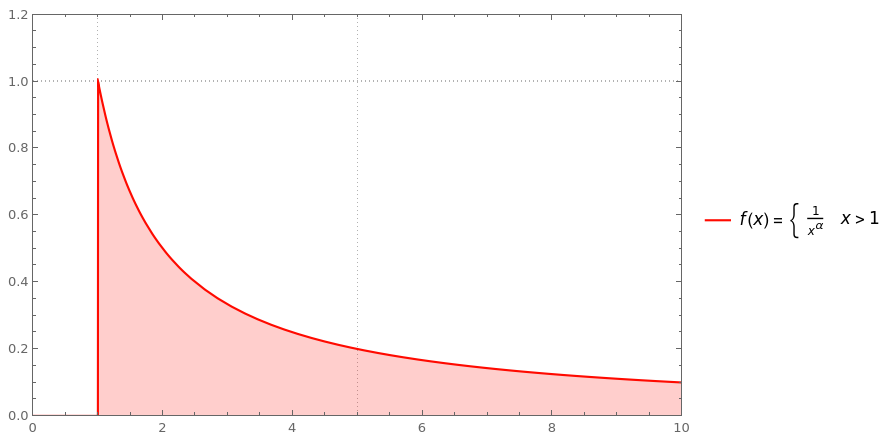
\includegraphics[width=\textwidth]{unosuxallaalpha.png}
\end{figure}

Fissato $c > 1$, riesco a definire $\int_{1}^{c} f(x)dx$ perchè integro una funzione limitata su un intervallo limitato.\\
Posso dunque definire
\begin{empheq}{align*}
	\int_{1}^{+\infty} f(x)dx &=\lim_{c\rightarrow +\infty} \int_{1}^{c}f(x)dx, \,\,\,\,\, \text{se}\,\,\, \exists\\
	\int_{1}^{+\infty} \frac{1}{x^\alpha} dx &= \lim_{c \rightarrow + \infty}\int_{1}^{c} \frac{1}{x^\alpha}dx\\
	&=
	\begin{cases}
		& \lim_{c \rightarrow +\infty}\frac{1}{1-\alpha}[c^{1-\alpha}-1]\,\,\,\, \text{se}\,\,\, \alpha \neq 1\\
		& \lim_{c \rightarrow +\infty} \ln c \,\,\,\, \text{se} \,\,\, \alpha=1
	\end{cases}\\
	&=
	\begin{cases}
		& \frac{1}{\alpha-1} \,\,\,\, \text{se} \,\,\, \alpha > 1\\
		&+\infty \,\,\,\, \text{se} \,\,\, \alpha \leq 1
	\end{cases}
\end{empheq}

\paragraph{\textcolor{red}{Esempio}}
\begin{empheq}{equation*}
	f(x)=-\ln x, \,\,\, x \in ]0,1]
\end{empheq}
e provo a definire 
\begin{empheq}{equation*}
	\int_{0}^{1} f(x)dx
\end{empheq}
cioè l'integrale di una funzione illimitata su un intervallo limitato.\\

\begin{figure}[h!]
	\centering
	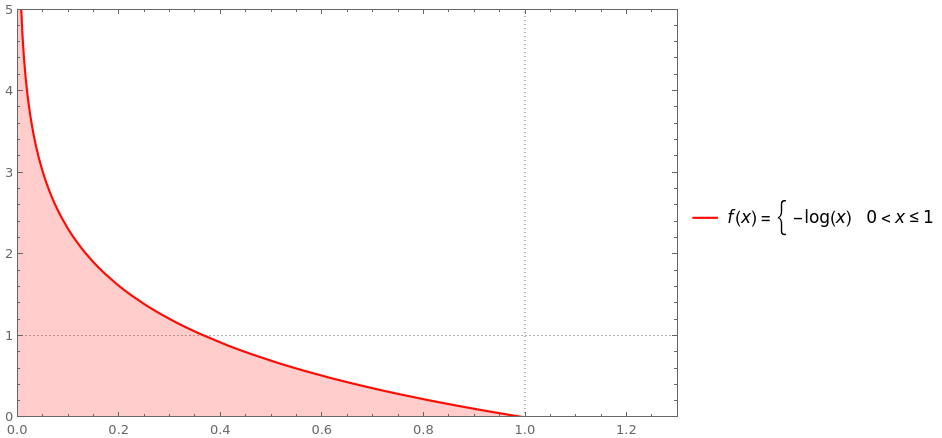
\includegraphics[width=\textwidth]{intda1a0.png}
\end{figure}
Riesco a definire bene $\int_{c}^{1} f(x)dx$ perchè integro una funzione limitata
\textcolor{orange}{$(|f(x)|\leq -\ln c \forall x\in[c,1])$} su un intervallo limitato.\\
Posso dunque definire
\begin{empheq}{align*}
	\int_{0}^{1} f(x)dx &= \lim_{c\rightarrow +0^+} \int_{c}^{1} f(x)dx\,\,\,\,\,\, \text{se}\,\,\, \exists\\
	\int_{0}^{1}(-\ln x) dx &= \lim_{c \rightarrow 0^+} \int_{c}^{1}(-\ln x)dx\\
	&= \lim_{c \rightarrow 0^+} [x-x\ln x]_{c}^{1} \\
	&= \lim_{c \rightarrow 0^+} [1-c+c\ln c]=1
\end{empheq}

\paragraph{\textcolor{red}{Definizione}}
Sia $f:[a,b[\rightarrow \R, a,b \in \R \cup\{+\infty\}$ \textcolor{orange}{(voglio definire $\int_{a}^{b}f(x)dx$)} Riemann integrabile in $[a,c]\,\, \forall c \in [a,b[$. Se $\exists$ finito il $\lim_{c \rightarrow b^-} \int_{a}^{c}f(x)dx $, allora $f$ si dice integrale in senso improprio o generalizzato in $[a,b[$ e la quantità 
\begin{empheq}{equation*}
	\int_{a}^{b} f(x)dx = \lim_{c\rightarrow b^-} \int_{a}^{c} f(x)dx
\end{empheq}
si dice integrale improprio o generalizzato di $f$ in $[a,b[$.\\
Analogamente, data $f:]a,b]\rightarrow \R, a,b \in \R \cup \{-\infty\}$, Riemann integrabile in $[c,b]\,\, \forall c \in ]a,b]$. Se $\exists$ finito il $\lim_{c \rightarrow a^+} \int_{c}^{b} f(x)dx$, allora $f$ si dice integrabile in senso improprio o generalizzato in $]a,b]$ e la quantità
\begin{empheq}{equation*}
	\int_{a}^{b} f(x)dx = \lim_{c \rightarrow a^+} \int_{c}^{b} f(x)dx
\end{empheq}
si dice integrale improprio o generealizzato di $f$ in $]a,b]$.\\
Se $f$ è integrabile in senso improprio in un intervallo $I$, allora si dice anche che l'integrale (improprio) di $f$ in $I$ è convergente o che $f$ ha integrale (improprio) convergente in $I$.\\
Se il limite che definisce l'integrale improprio di $f$ è infinito, si dice anche che l'integrale (improprio) di $f$ è divergente o che $f$ ha integrale (improprio) divergente in $I$.

\paragraph{\textcolor{red}{Osservazione}}
Vista la definizione, 
\begin{empheq}{equation*}
	\int_{1}^{+\infty}\frac{1}{x^\alpha}dx \,\,\,\,\, \text{converge} \Leftrightarrow \alpha > 1
\end{empheq}

\paragraph{\textcolor{red}{Esempio Importante}}
\begin{empheq}{equation*}
	f(x)=\frac{1}{(x-a)^\alpha}, \,\,\,\, x \in ]a,a+1], \,\,\, a\in \R \,\, \text{fissato},\,\,\, \alpha\in\R\,\,\, \text{parametro},\,\,\, \alpha > 0
\end{empheq}
Studiamo la convergenza di 
\begin{empheq}{align*}
	\int_{a}^{a+1} \frac{1}{(x-a)^\alpha} dx  &= \lim_{c \rightarrow a^+} \int_{c}^{a+1} \frac{1}{(x-a)^\alpha} dx\\
	&=
	\begin{cases}
		& \lim_{c \rightarrow a^+} \frac{1}{1-\alpha}[1-(c-a)^{1-\alpha}] \,\,\,\, \text{se}\,\, \alpha \neq 1 \\
		& \lim_{c \rightarrow a^+} -\ln(c-a)\,\,\,\, \text{se} \,\, \alpha =1
	\end{cases}\\
	&=
	\begin{cases}
		& \frac{1}{1-\alpha} \,\,\,\, \text{se}\,\, \alpha <1 \\
		&+\infty \,\,\,\, \text{se}\,\, \alpha \geq1.
	\end{cases}
\end{empheq}
Dunque 
\begin{empheq}{equation*}
	\int_{a}^{a+1} \frac{1}{(x-a)^\alpha} dx \,\,\,\, \text{converge} \Leftrightarrow \alpha < 1.
\end{empheq}
In particolare
\begin{empheq}{equation*}
	\int_{0}^{1} \frac{1}{x^\alpha} \,\,\,\, \text{converge} \Leftrightarrow \alpha < 1.
\end{empheq}

\paragraph{\textcolor{red}{Esempio}}
Stabilire se converge 
\begin{empheq}{equation*}
	\int_{0}^{1} \frac{\sin{\frac{1}{x}}}{x^2} dx
\end{empheq}
\begin{figure}[h!]
	\centering
	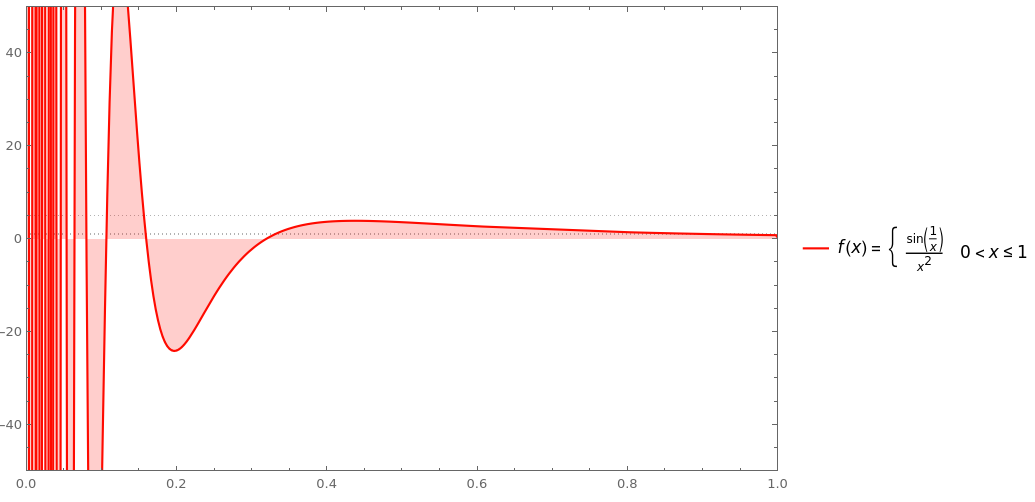
\includegraphics[width=\textwidth]{senobuffo.png}
\end{figure}

Devo calcolare 
\begin{empheq}{equation*}
	\lim_{c\rightarrow0^+} \int_{c}^{1} \frac{\sin{\frac{1}{x}}}{x^2} dx= \lim_{c \rightarrow 0^+} \cos{\frac{1}{x}}|_{c}^{1}=\lim_{c\rightarrow 0^+}\left(1-\cos{\frac{1}{c}}\right)
\end{empheq}
che non esiste $\Rightarrow$ la funzione $f(x)=\frac{\sin{\frac{1}{x}}}{x^2}$, non è integrabile in senso improprio in $]0,1]$.

\paragraph{\textcolor{red}{Esempio Importante}}
\begin{empheq}{align*}
	\int_{0}^{+\infty} e^{\alpha x} dx &=\lim_{c \rightarrow +\infty} \int_{0}^{c} e^{\alpha x} dx \\&= \lim_{c \rightarrow +\infty} \frac{1}{\alpha}(e^{\alpha c}-1)\\
	&= \begin{cases}
		& -\frac{1}{\alpha} \,\,\,\, \text{se} \,\, \alpha <0\\
		&+\infty \,\,\,\, \text{se} \,\, \alpha >0.
	\end{cases}
\end{empheq}
\begin{empheq}{equation*}
	\int_{0}^{+\infty} e^{\alpha x} \,\,\,\,\, \text{converge} \Leftrightarrow \,\,\, \alpha <0.
\end{empheq}
Analogamente
\begin{empheq}{equation*}
	\int_{-\infty}^{0} e^{\alpha x} dx \,\,\,\,\, \text{converge} \Leftrightarrow \,\,\, \alpha > 0.
\end{empheq}
Dato $ a>0$, scrivendo $e^{\alpha x} = e^{(\alpha \ln a)x}$ si deduce la convergenza degli integrali
\begin{empheq}{align*}
	&\int_{-\infty}^{0} e^{\alpha x} dx \\
	&\int_{0}^{+\infty}  e^{\alpha x} dx.
\end{empheq}
\text{\textcolor{orange}{(Facile esercizio per casa)}}

\paragraph{\textcolor{red}{Nota Bene}}
$f:[1,+\infty[ \rightarrow \R$ continua. E' vero o falso che $\lim_{x \rightarrow +\infty} f(x)=0 \Rightarrow \int_{1}^{+\infty} f(x)dx$ converge?\\
E' falso!!! Si veda $f(x)=\frac{1}{x}$\\
E' vero o falso che
$\int_{1}^{+\infty}f(x) dx$ converge $\Rightarrow \lim_{x \rightarrow +\infty} f(x)=0$?\\
E' falso!!!\\
\begin{figure}[h!]
	\centering
	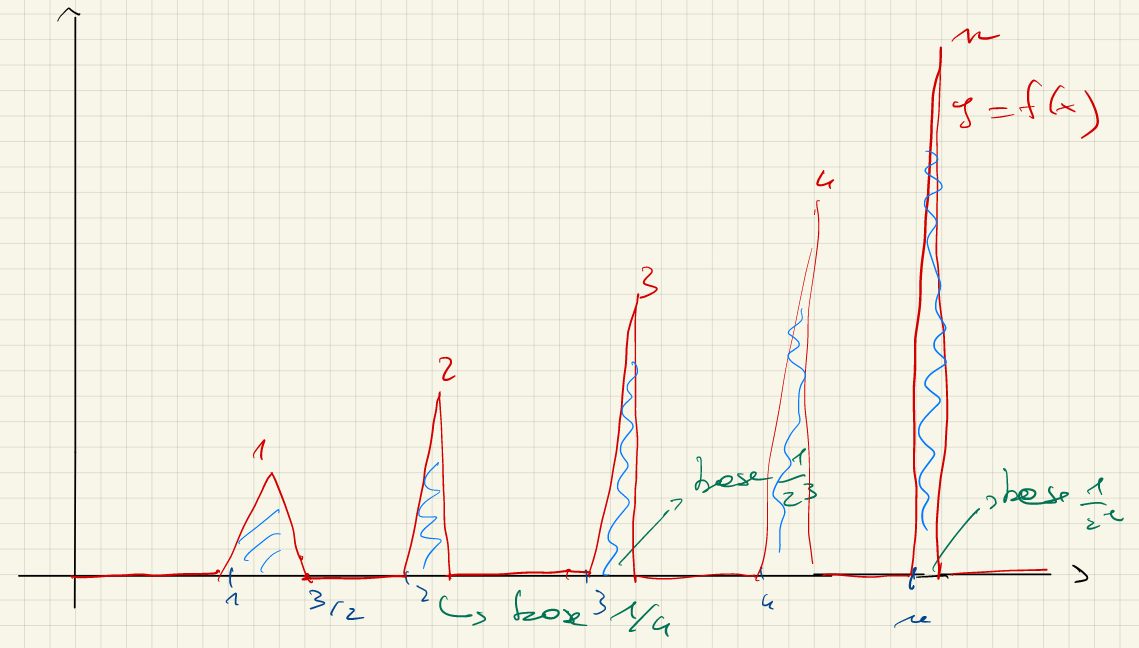
\includegraphics[width=\textwidth]{cosiappuntiti.png}
\end{figure}

Ad ogni numero naturale $n$ costruite un triangolo di base $\frac{1}{2^n}$ e altezza $n$

\begin{empheq}{equation*}
	\int_{1}^{+\infty} f(x)dx = \sum (\text{aree dei triangoli}) = \sum_{n=1}^{\infty} \frac{1}{2} \frac{1}{2^n} \cdot n = \frac{1}{2} \sum_{n=1}^{\infty} \frac{n}{2^n}, 
\end{empheq}
che è una serie convergente.

\paragraph{\textcolor{red}{Osservazione}}
Se $f:[a,b] \rightarrow \R$ è Riemann integrabile, allora è integrabile anche in senso improprio e i due integrali coincidono.

\paragraph{\textcolor{red}{Definizione}}
$f:[a,b] \rightarrow \R,\,\, a,b \in \R \cup \{\pm \infty\}$, Riemann integrabile in $[c,d]\,\, \forall a<c<d<b$. $f$ si dice integrabile in senso improprio in $ ]a,b[$ se, fissato $\xi \in ]a,b[$, lo è in $]a, \xi]$ e in $[\xi,b[$ \textcolor{orange}{(esistono finiti $\lim_{c \rightarrow a^+} \int_{c}^{\xi} f(x)dx$ e $\lim_{d\rightarrow b^-}\int_{\xi}^{d} f(x)dx$)} e in tal caso si pone 
\begin{empheq}{equation*}
	\int_{a}^{b} f(x)dx = \int_{a}^{\xi} f(x)dx + \int_{\xi}^{b} f(x) dx
\end{empheq}
Si verifica che la definizione non dipende da punto $\xi$ fissato.


\paragraph{\textcolor{red}{Esempio}}
Come si integra $\int_{-\infty}^{+\infty} \frac{1}{1+x^2}dx$?\\
$x \mapsto \frac{1}{1+x^2}$ è integrabile secondo Riemann in $[c,d] \,\, \forall c<d$. \\
Sia $\xi = 2$. Dobbiamo verificare se la funzione è integrabile in senso improprio in $]-\infty,2] $ e in $ [2, +\infty[$
\begin{empheq}{align*}
	&\int_{-\infty}^{2}\frac{1}{1-x^2}dx = \lim_{c \rightarrow -\infty} \int_{c}^{2} \frac{1}{1+x^2}dx = \lim_{c \rightarrow -\infty} \left(\arctan{2+\frac{\pi}{2}}\right)= \arctan{2+\frac{\pi}{2}}\\
	&\int_{2}^{+\infty}\frac{1}{1-x^2} dx =\lim_{c \rightarrow +\infty} \int_{2}^{c} \frac{1}{1-x^2}dx=\lim_{c \rightarrow +\infty} (\arctan{c}-\arctan{2})=\frac{\pi}{2}-\arctan{2}\\
	&\Rightarrow \int_{-\infty}^{+\infty} \frac{1}{1+x^2}dx \,\,\,\, \text{converge e}\,\,\, \int_{-\infty}^{+\infty}\frac{1}{1+x^2}dx = \int_{-\infty}^{2}\frac{1}{1+x^2} dx+ \int_{2}^{+\infty}\frac{1}{1+x^2}dx
\end{empheq}

\paragraph{\textcolor{red}{Esempio}}
\begin{empheq}{align*}
	&f(x)=\frac{1}{x^\alpha}, \,\,\,\,\,x \in ]0,+\infty[\\
	&\alpha > 0 \Rightarrow \lim_{x \rightarrow 0^+} f(x)=+\infty.
\end{empheq}
Preso $\xi=1$, $f$ è integrabile in senso improprio in $]0,+\infty[ \Leftrightarrow$ entrambi gli integrali $\int_{0}^{1} \frac{1}{x^\alpha} dx$ e $\int_{1}^{+\infty} \frac{1}{x^\alpha} dx$ convergono ma
\begin{empheq}{align*}
	&\int_{0}^{1}\frac{1}{x^\alpha}dx \,\,\,\,\, \text{converge} \Leftrightarrow \alpha <1 \\
	& \int_{1}^{+\infty} \frac{1}{x^\alpha}dx \,\,\,\,\, \text{converge} \Leftrightarrow \alpha > 1\\
	& \Rightarrow \int_{0}^{+\infty} \frac{1}{x^\alpha}dx \,\,\,\text{non converge per alcun valore di} \,\, \alpha
\end{empheq}

\paragraph{\textcolor{red}{Esempio}}
\begin{empheq}{equation*}
	f(x)= 
	\begin{cases}
		& e^x\,\,\,\,\, \text{se} x \leq 1 \\
		& \frac{1}{x \sqrt{x-1}}\,\,\,\,\, \text{se}\,\,\, x>1
	\end{cases}
\end{empheq}
vogliamo stabilire se $\int_{-\infty}^{+\infty}f(x)dx$ converge.\\
\begin{figure}[h!]
	\centering
	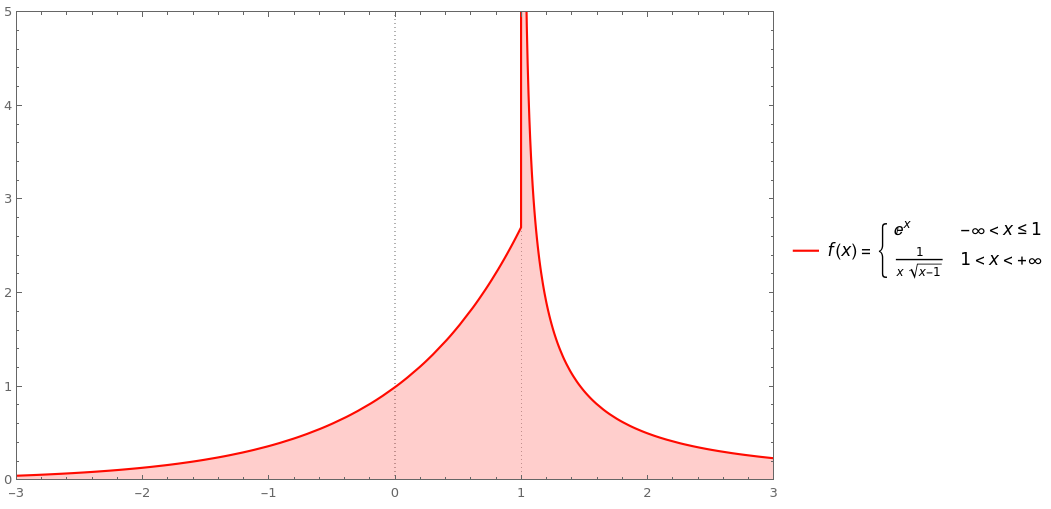
\includegraphics[width=\textwidth]{espefrac.png}
\end{figure}

Devo studiare $\int_{-\infty}^{1}f(x) dx = \int_{-\infty}^{1}e^x dx$ e, prendendo $\xi=3$,  $\int_{1}^{3}f(x)dx$ e $\int_{3}^{+\infty}f(x)dx$. Se tutti convergono, anche $\int_{-\infty}^{+\infty} f(x)dx$ converge e 
\begin{empheq}{equation*}
	\int_{-\infty}^{+\infty} f(x)dx = \int_{-\infty}^{1} f(x)dx + \int_{1}^{3} f(x)dx + \int_{3}^{+\infty} f(x)dx
\end{empheq}

\paragraph{\textcolor{red}{Ulteriore Definizione}}
In generale, data $f:]a,b[\rightarrow \R$ integrabile in senso improprio in $]x_0,x_1[,]x_1,x_2[,...,]x_{n-1},x_n[$ con $a= x_0 <x_1<...<x_n=b$, allora $f$ si dice integrabile in senso improprio in $]a,b[$ e si pone 
\begin{empheq}{equation*}
	\int_{a}^{b}f(x)dx= \sum_{i=1}^{n} \int_{x_{i-1}}^{x_i}f(x)dx.
\end{empheq}



\end{comment}